\documentclass[11pt]{article}
\usepackage[a4paper, hmargin={2.8cm, 2.8cm}, vmargin={2.5cm, 2.5cm}]{geometry}
\usepackage{eso-pic}
\usepackage{graphicx}
\usepackage{placeins}
\usepackage{amsmath}
\usepackage[utf8]{inputenc}
\usepackage[T1]{fontenc}
\usepackage{verbatim}
\usepackage[all]{xy}
\usepackage{amssymb}
\usepackage{listings}
\usepackage{glossaries}
\usepackage{hyperref}
\usepackage{multicol}
\usepackage{color}
\usepackage{url}
\usepackage{tcolorbox}
\usepackage{enumerate}
\usepackage{caption}
\usepackage{subcaption}
\usepackage{float}
\usepackage{pdflscape}
\usepackage{amsthm}

\newacronym{POS}{POS}{Parts-of-Speech}
\newacronym{ISG}{ISG}{Integrated Syntactic Graph}
\newacronym{UBM}{UBM}{Universal Background Model}
\newacronym{AGS}{AGS}{Average Group Similarity}
\newacronym{AUROC}{AUROC}{Area Under Receiver Operating Characteristic}
\newacronym{ROC}{ROC}{Receiver Operating Characteristic}
\newacronym{SCAP}{SCAP}{Source Code Author Profile}
\newacronym{CNG}{CNG}{Common n-gram}
\newacronym{LNG}{LNG}{Local n-gram}
\newacronym{RLP}{RLP}{Recentred Local Profiles}
\newacronym{KNN}{KNN}{K-Nearest Neighbours}
\newacronym{SVM}{SVM}{Support Vector Machine}
\newacronym{NLP}{NLP}{Natural Language Processing}
\newacronym{CNN}{CNN}{Convolutional Neural Network}
\newacronym{RNN}{RNN}{Recurrent Neural Network}
\newacronym{AA}{AA}{Authorship Attribution}
\newacronym{AV}{AV}{Authorship Verification}
\newacronym{GRU}{GRU}{Gated Recurrent Unit}
\newacronym{LSTM}{LSTM}{Long Short Term Memory}
\newacronym{ReLu}{ReLu}{Rectified Linear Unit}
\newacronym{SRP}{SRP}{Studieretningsprojekt}

\newacronym{TP}{TP}{True Positive}
\newacronym{TN}{TN}{True Negative}
\newacronym{FP}{FP}{False Positive}
\newacronym{FN}{FN}{False Negative}
\newacronym{TPR}{TPR}{True Positive Rate}
\newacronym{TNR}{TNR}{True Negative Rate}
\newacronym{FPR}{FPR}{False Positive Rate}
\newacronym{FNR}{FNR}{False Negative Rate}

\theoremstyle{plain}
\newtheorem{definition}{Definition}[section]

\author{
    \begin{tabular}{ccc}
    \Large{August V. S\o rensen} & \& & \Large{Magnus N. Stavngaard} \\
    august.vinkel@gmail.com      &    & magnus@stavngaard.dk         \\
    NCB360                       &    & MZC887
    \end{tabular}
}



\title{
    \vspace{3cm}
    \Huge{Authorship Verification} \\
    \Large{Deep Learning Based Methods for Authorship Verification}
}

\usepackage{fancyhdr}
\pagestyle{fancy}

\lhead{University of Copenhagen}
\rhead{August V. S\o rensen \& Magnus N. Stavngaard}
%\cfoot{}
%\rfoot{\thepage}

\begin{document}

    \AddToShipoutPicture*{\put(0,0){\includegraphics*[viewport=0 0 700 600]{pictures/report/ku-farve}}}
    \AddToShipoutPicture*{\put(0,602){\includegraphics*[viewport=0 600 700 1600]{pictures/report/ku-farve}}}
    \AddToShipoutPicture*{\put(0,0){\includegraphics*{pictures/report/ku-en}}}
    \clearpage\maketitle
    \thispagestyle{empty}
    \newpage

    \pagenumbering{roman}
    \setcounter{page}{1}

    \begin{abstract} \label{sec:abstract}

    In this thesis we investigate authorship verification of texts produced by
    secondary school students. Authorship verification or \textit{ghost writer
    detection} is the process of determining whether a text is written by an
    author given a set of texts written by the same author. We work with the
    Danish company MaCom that provides a dataset containing assignments from
    secondary school students. We focus on deep neural networks to perform the
    authorship verification. We implement two baseline methods representing
    classic machine learning solutions to the authorship verification problem.
    After that we present three networks to solve the same problem:

    \begin{itemize}

        \item

            A convolutional neural network working on the character level of the
            texts,

        \item

            A recurrent neural network working on the sentence level of the
            texts,

        \item

            A convolutional neural network working on the character and word
            level of the texts.

    \end{itemize}

    Classic machine learning methods for authorship verification use manually
    chosen feature configurations. The networks we implement extract features
    from raw text data. The networks beat both of the baseline methods on all
    relevant parameters. On a dataset with 50\% ghost written assignments we
    achieve an accuracy of 86.5\%.

    Our methods are meant to be used in a supporting manner for teachers of
    secondary schools for detecting ghost written assignments. We are able to
    give teachers feedback on why the networks makes a decision and we are able
    to detect specific areas of assignments that might be ghost written.

\end{abstract}


    \newpage
    \tableofcontents
    \newpage

    \pagenumbering{arabic}
    \setcounter{page}{1}

    % Introduction should be written in the present tense!
%
% Your introduction needs to include background information which is generally
% accepted as fact in a discipline. You also need to explain why the research
% you are reporting is important. It is usually presented in the present tense.
%   - https://services.unimelb.edu.au/__data/assets/pdf_file/0009/471294/Using_tenses_in_scientific_writing_Update_051112.pdf

\section{Introduction} \label{sec:introduction}

% An introduction to the context or background of the topic (you could include
% interesting facts or quotations)

In this thesis we work on the problem of authorship verification using texts
written by Danish secondary school pupils. Authorship verification and
authorship attribution is the ability to distinguish between authors of texts
based on a set of extracted textual features. The automation of authorship
attribution/verification has been a lively branch of research ever since the
beginning of the digital age, giving birth to online digital text forensics
tasks, such as the work by \citet{pan:2015}. Initial attempts at quantifying
writing style can be seen in \citet{Mendenhall237}, who attempted to determine
the authorship of several of Shakespeare's texts. There is a theory that
Shakespeare did not write some or all of his texts, or that he was a synonym
for one of more more unknown authors. \citet{Mendenhall237} attempted this
classification using the frequency distribution of words of different lengths.
Throughout the years the approaches to this problem have changed quite a bit.
When authorship attribution started to interest researchers the approaches were
Stylometric i.e. they were based on the linguistic style of authors. In addition
to that, fully automated systems were rare and was mostly used in a supporting
manner. It was during the 1990's that fully automated systems became more
prevalent. The main reason for this was the Internet. Before the Internet, the
data available simply was not suitable for authorship attribution tasks. Books
were too big, resulting in a lack in homogeneity, and the amount of authors and
bench-marking data was too small. The Internet paved the way for insurmountable
amounts of data and variations of that data, impacting areas such as information
retrieval, machine learning and \gls{NLP}.

In order for any fully automatic authorship verification to work, stylometric
features describing the text has to be automatically extracted. These features
span multiple linguistic layers, ranging from the low level character n-grams
to the high level application specific features such as text creation date and
number of edits. Many of the current day state-of-the-art approaches are based
on these features.

% The reason for writing about this topic:

We want to experiment with and solve an authorship verification task for the
Danish company \texttt{MaCom A/S} \footnote{\url{http://www.macom.dk/}}.
MaCom is the company behind the product \texttt{Lectio}
\footnote{\url{https://www.lectio.dk/}}, which is a website that allows for
student administration, communication, and digital teaching aid. Lectio is used
in schools all over Denmark. A service the website offers is the submission
and handling of assignments written by students throughout their enrollment.
MaCom has shown interest in determining whether or not these assignment
were written by someone other than the student (a ``ghost writer''). Ghost
writing is especially a problem on the \gls{SRP} assignment. \gls{SRP} is
an interdisciplinary assignment all Danish secondary school students turn
in at the end of their third year. There is no oral examination for the
assignment and the grade obtained is part of the students final results from
the secondary school. The combination of the importance of the assignment
and no oral examination leads to students turning in assignments written by
ghost writers. The Danish state owned public service radio and television
company \texttt{DR} has written an article describing the ghost writer problem
\footnote{\url{https://www.dr.dk/nyheder/indland/elever-bruger-ghostwritere-til-
eksamen}}. The article describes that when asking 2000 student, 58\% got help
from friends or family, and around 15\% knew someone who had their assignment
written by someone else. In this thesis we setup a system for detecting ghost
writing based on machine learning methods. The system is meant to help teachers
make decisions about whether or not an assignment turned in by a student is
written by someone else. It is not important that the system catches 100\% of
the assignments written by someone else. If the system only catches a fraction
of the cheaters, it will deter other students from cheating. What is most
important is that the system does not accuse anyone of cheating who has turned
in their own assignment. The system should also be able to give evidence for why
we think a particular assignment is written by someone else. Such evidence could
for example be that the frequency of particular words is significantly different
in the new assignment than in all previously handed in by the student. Evidence
for why we think an assignment is written by someone else will help a teacher if
he/she wants to accuse a student of using a ghost writer.

% Introduce the main ideas that stem from your topic/title and the order in
% which you will discuss them?

As described the problem main problem we try to solve in this thesis is
authorship verification which is defined below.

\begin{definition}[Authorship Verification]
    \label{def:authorship_verification}

    Given a set of texts $T_\alpha$ written by author $\alpha$ and a single
    text $x$ of unknown authorship, determine if $x \in T_\alpha$.

\end{definition}

Authorship verification is closely linked with the problem of authorship
attribution as can be seen in the definition of authorship attribution shown
below.

\begin{definition}[Authorship Attribution]

    Given a set of authors $\mathcal{A} = \{ \alpha_1, \alpha_2,...\alpha_N\}$,
    each with set of text $T_{\alpha_i}$, and a text of unknown authorship
    \texttt{x}, determine which $\alpha_i \in \mathcal{A}$ is the author of
    \texttt{x}.

\end{definition}

The problems are closely linked since an answer for authorship attribution
can be obtained by using authorship verification and an answer for authorship
verification can be obtained by using authorship attribution. Consider a case
where we are given an oracle answering the authorship verification problem
$\mathcal{S}$. $\mathcal{S}$ is a mapping from an author $\alpha$ and text
$x$ to either true or false. Given an instance of the authorship attribution
problem with authors $\mathcal{A}$ and text $x$ we solve the problem by using
$\mathcal{S}$ on each author $\alpha \in \mathcal{A}$. We return the author
where $\mathcal{S}$ reports true. Now consider a case where we are given a
solution to the authorship attribution problem $\mathcal{S}'$. $\mathcal{S}'$
is now a mapping from a set of authors $\mathcal{A}$ and text $x$ to an author
$\alpha \in \mathcal{A}$. Given an instance of the authorship verification
problem with author $\alpha_i \in \mathcal{A}$ and text $x$ and a set of texts
written by different authors $\overline{T}_{\alpha} = \bigcup_{\beta \in A
\setminus \{\alpha\}} T_\beta$ we solve the verification problem by applying the
attribution function to the texts $T_{\alpha} \cup \overline{T}_{\alpha}$ and
the text of unknown authorship $x$. If $x \in T_{\alpha}$ we report true and
otherwise false.

    \FloatBarrier

    \section{Related Work} \label{sec:related_work}
%The problem of authorship verification


The method implemented by \cite{shrestha2017}, was their attempt at \gls{AA}
on short texts. The reasoning behind the only focusing on short texts was the
advent of social media, and the great usage of E-mail. Their approach makes use
of a \gls{CNN}. This \gls{CNN} only takes in a sequence of character-n-grams.
The reasoning for this usage of only char-n-grams was the small amount of text
in each sample. By passing these N-grams through a Embedding layer, a 25\%
dropout layer, 3 convolutional layers and then using max-over-time, they get
a compact representation of the text. They hypothesize this representation
captures the morphological, lexical and syntactic level of the supplied text.
This compact representation is then parsed through a fully connected soft-max
layer, to produce a probabilistic distribution over all authors. In order to
test their method they made use of a twitter data set, containing approximately
9000 user, all having over a 1000 tweets to their name. They made use of two
different configurations of their networks. One using character-1-grams and one
using character-2-grams. After removing bot-like authors, they got an accuracy
of 0.678, and 0.683 respectively. This however, was only with 35 authors used,
and 1000 tweets per author. In the case where either the authors count was
increased or the number of tweets was decreased, the accuracy quickly worsened.
In order to extract some sort of meaning from the predictions they made using
this approach, they made use of the saliency score to determine the impact each
n-gram had on the final decision.

    \FloatBarrier

    \section{Method} \label{sec:method} 

In this section we will describe the method we have used to solve the Authorship
Verification problem presented. In general there are two methods of representing
each author. There is the instance based approach and the profile based
approach. In the instance based approach each author is represented by a set of
texts they have written while in the profile based approach they are represented
by the sum of the set of texts they have written. The instance based approach is
illustrated in Figure \ref{fig:instance_based} and the profile based approach is
illustrated in Figure \ref{fig:profile_based}.

\begin{figure}[htb]
    \centering
    \textbf{Instance Based Authorship Verification or Authorship Attribution}
    \includegraphics[scale=0.5]{./pictures/method/InstanceBased.png}

    \caption{Illustrate the typical instance based Authorship Verification or
    Authorship Attribution solution setup. Inspired by \cite{stamatos2009} a
    set of authors are given as input each with a set of texts. Some Machine
    Learning model is trained on the input texts and the model is used to
    predict an unknown text. }

    \label{fig:instance_based}
\end{figure}

\begin{figure}[htb]
    \centering
    \textbf{Profile Based Authorship Verification or Authorship Attribution}
    \includegraphics[scale=0.5]{./pictures/method/ProfileBased.png}

    \caption{Illustrate the typical profile based Authorship Verification or
    Authorship Attribution setup. Inspired by \cite{stamatos2009} the texts of
    each author are combined using some combination function such as an average
    or a concatenation. Those \textit{profiles} are then given to a Machine
    Learning model to train. The output is a model which is used to predict
    unknown texts. }

    \label{fig:profile_based}
\end{figure}

We will generally use the instance based approach. The reason we use an instance
based approach is that it allows us to use extra information from each single
text. For example writing style may change over time especially for secondary
school pupils that evolve very much in a short amount of time. Since we use an
instance based approach we are able to weight similarity to newer texts higher
than similarity to older texts.

There are also another split between methods that we consider. There are
generalizing and author specific models. In a generalizing model only a single
model is trained on data from multiple authors and are able to make predictions
about previously unseen authors. In the author specific model a separate model
has to be trained for each author and is not able to make predictions for
previously unseen authors. The generalizing model has several advantages, it
only has to be trained once and after that it can be used for everyone and
it can make use of big data since it can use data from several authors for
training. The author specific model has the advantage that it can better fit
to the specific quirks of a particular author since it is trained separately
for each author. The downside of the author specific approach is that a new
model has to be trained for each new author. We will focus on the generalizing
approach since it is easier to implement for MaCom as they only have to train a
model once.

As a unit of measuring the quality of our models, and how well they adhere to
95\% specificity constraint, we will also compute the number of \gls{TP}s,
\gls{TN}s, \gls{FP}s and \gls{FN}s, as was done in a project previously created
by us.\cite{US} In these problems we get,

\begin{itemize}
    \item a \gls{TP} whenever we answer \textit{True} and the texts are written
        by the same author,
    \item a \gls{TN} whenever we answer \textit{False} and the texts are
        \textbf{not} written by the same author,
    \item a \gls{FP} whenever we answer \textit{True} and the texts are
        \textbf{not} written by the same author,
    \item a \gls{FN} whenever we answer \textit{False} and the texts are written
        by the same author.
\end{itemize}

Given those definitions the \gls{TPR}, \gls{FPR}, \gls{TNR} and \gls{FNR}
describes.

\begin{description}
    \item[\gls{TPR}: ] The fraction of positives that we reported \textit{True}
        on i.e. the fraction of texts written by the same author that we say are
        written by the same author.
    \item[\gls{FPR}: ] The fraction of negatives that we reported \textit{True}
        on i.e. the fraction of texts written by different authors that we say
        are written by the same author.
    \item[\gls{TNR}: ] The fraction of negatives that we reported \textit{False}
        on i.e. the fraction of texts written by different authors that we say
        are written by different authors.
    \item[\gls{FNR}: ] The fraction of positives that we reported \textit{False}
        on i.e. the fraction of texts written by the same author that we say are
        written by different authors.
\end{description}

And they can be computed as,

\begin{align}
    TPR &= \frac{TP}{TP + FN}, \\
    FPR &= \frac{FP}{FP + TN}, \\
    TNR &= \frac{TN}{TN + FP}, \\
    FNR &= \frac{FN}{FN + TP}.
\end{align}

In the case of MaCom, we want to minimize the \gls{FNR} as much as possible, so
as to not wrongfully accuse anyone of not having written their assignment.


\subsection{Deep Learning}

In this paper we will approach the authorship verification/attribution problem
using deep-learning. The term deep learning, was first introduced to
machine machine learning in 1989, and afterward to \gls{NN}'s in 2000. The terms
quickly became synonymous with \gls{NN}'s due to them being some of the more
efficient deep learning methods.\cite{Schmidhuber:2015}

With the inner workings of the brain used as the basis, a standard simple
\gls{NN} consists of a set interconnected processors, called neurons. Each of
these neurons has a real-valued activation associated with it, which activates
differently depending on the specific neuron. The input neurons activate through
perceiving the environment, or in other words, when it is fed data externally.
Other neurons are simply activated through the weighted activation of previous
neurons. More details regarding these weights will be presented later in the
paper.\cite{DBLP:journals/corr/Schmidhuber14}

\gls{NN}'s have been around since the 1940's. However, back then they were
merely variations of the linear regressors used at the time, and wasn't
very reminiscent of the Networks on can see today. It wasn't until the
late 1960's, early 70's, that networks comparable to the more modern
approaches surfaced. Examples of such early works, are the two publications
\cite{ivakhnenko1973cybernetic} and \cite{4308320}, which describe multi-layered
feed-forward supervised neural network architectures. While the work described
in \cite{4308320} was indeed one of the first cases of the modern \gls{NN},
actually getting the network to learn was still a problem, as the tweaking of
individual weights attributed to each neuron in the network wasn't trivial.
Little did they know, research to solve that problem was already in progress.
The basics of continuous \gls{BP} was initially described in 1960, in
\cite{Kelley1960}, quickly followed by a simpler approach which used only the
chain rule in 1962, \cite{DREYFUS196230}. It wasn't until 1970 that the modern
version of \gls{BP} was described, using automatic differentiation as its
basis. With this, the increase in research of usages of \gls{BP} increased the
following decades. As the computational power increased several 1000 folds in
the 90's and 2000's, so did the practical usage of \gls{BP}, and \gls{NN} in
general\cite{Schmidhuber:2015}. The real life application of \gls{BP}, will be
described in section \ref{sec:BP}

Like with the history of authorship attribution, research in this area of
science picked up more interest, as we entered the modern computational age,
and with the introduction of the \gls{CNN}. \gls{CNN}s bases themselves on
the early work described in \cite{TJP:TJP19681951215}. They showed that cats
and monkeys visual cortexes contain a set of neurons, each individually
responding to a receptive field, or area, of their field of view. Neighboring
receptive fields all have a certain amount of overlap, however in the end
a cohesive view is created. This is what paved the way for neocognition in
1980\cite{Fukushima1980}, the basis of \gls{CNN}'s, which works in a very
similar manner, looking at overlapping subsections of data. These convolutional
neurons however were rarely used alone, but together with a down-sampling neuron
such as Max Pooling introduced in 1993.\cite{Schmidhuber:2015}

\subsubsection{Neurons}

As mentioned previously a \gls{NN} consists of a collection of neurons. Each
neuron is a simplified mathematical model, which behaves much like neurons in
the brain would, receiving, processing and transmitting data/information. Each
neuron has a set of inputs called $x_i$ and a single output called $z_i$. The
neurons compute a weighted sum of its inputs and applies an activation function
$h$ to the weighted sum. The weights are called $w_i$. The function each neuron
computes is then,

\begin{equation}
    z_i = h\left(
        \sum_{i = 1}^d w_ix_i + w_0
    \right).
\end{equation}

The training of a \gls{NN} consists of changing the weights applied at each
neuron, with the goal of modeling the relationships present in the data.

\subsubsection{TODO: Backpropagation}\label{sec:BP}
The actual modeling and learning that the \gls{NN} does, can be attributed
to \gls{BP}. It by this process, that the weight in our \gls{NN} are updated,
signifying the learning the network does. The process can be split into three
steps, which are continuously repeated:

\begin{enumerate}
    \item Feed Forward
    \item Back Propagate
    \item Update Weights
\end{enumerate}

The goal of these three steps is to minimize the overall cost of the network.
The cost in this case, refers to the loss we end up with. In order to that the
network makes use of the gradient to optimize each of the individual weights.
Step 1, feeding forward, is simply a parse through the \gls{NN}. When this is
done we can compute the cost of that single training example. Looking at each
of the previous contributing nodes, we can attempts to minimize the final cost
of the network by tweaking the weights, using the gradient of the activation
function of that particular layer, with respect to those weights. Doing this
iteratively throughout the network is back propagation, as we are propagating
the loss of that single value back throughout the network. In the end, each
single training sample would have a desired change to each of the weights.
These desired changes would then be averaged and applied to the weights of the
network. This approach however, is very cost ineffective in terms of computing
power. As such the practical application of this entails shuffling and dividing 
your training data into batches, and doing the 3 steps listed above for each of
the batches. This results in a very good approximation of the ideal weights,
without spending as much computational time.


TODO: More math!


\subsubsection{Activation Functions}
The activation function $h$, used at each neuron, defines the output of the
node given a certain input. A simple example of this would be computer chip
circuit, which can be seen as a series of activation functions outputting 0 or
1 depending on their input. This activation function would be a linear one.
When applying activation functions to neurons in \gls{NN}s, they are usually
non-linear, as it allows for the computation of more complex problems using a
smaller amount of neurons, relative to usage of a linear activation function,
as they allow for the universal function approximation, a point also made by
\cite{6797088}

A plot of different activation functions is shown in Figure
\ref{fig:activation_functions}.

\begin{figure}
    \centering
    \textbf{Activation Functions}\par\medskip
    \includegraphics[width=0.5\textwidth]{./pictures/method/activation_functions.png}
    \caption{Different activation functions that can be used in neural
        networks.}
    \label{fig:activation_functions}
\end{figure}

Each activation function has its pros and cons. We mainly made use of the
\gls{ReLu} activation function in the hidden layers of our networks. The
reason for this selection is its general purpose use. When selecting an
activation function for your neurons, the best function would be the one which
best approximates the underlying function. Without a good idea as to what
that function might be, \gls{ReLu} is a good starting point. Its simplicity
provides a quick computation time, and its below zero limitation means that a
large portion of the network won't be activating, resulting in an even smaller
computation time. In addition to that, the derivative of the function is 1
in the case of a positive input, resulting in the \gls{BP} loss having equal
influence throughout the network. In the case of other activation functions,
this might not be the case, resulting in an altering of the error as we
propagate backwards through the network. This could lead to a big error in the
deeper layers not reaching the shallow layers of the network. This property of
the \gls{ReLu} activation function, does however not come without its costs.
If the learning rate of the network isn't configured correctly, a \gls{ReLu}
activated neuron might be blasted with a gradient so large, that it never
reaches a point of activation again. In other words, the neuron "dies". As
such, one can risk a network containing a lot of dead non-activation neurons,
thus greatly decreasing its quality. On the other hand the sigmoid function,
doesn't allow its neurons to die. It can become victim to saturation. In
the case of weight being too small or too high, the output values will be
placed at the far ends of the sigmoid range of values. At this point the
gradient is incredibly small, meaning that the contribution that neuron now has
is negligible. This neuron is now only a strain on the network, slowing it
down through its activation, but contribution nothing, a problem \gls{ReLu}
does not have. Its based on these considerations we chose the \gls{ReLu}
activation function, leaving us the task of properly selecting our learning
rate.\cite{JiYan, AndrejKarpathy, AvinashSharmaV}

As the activation function of our output neurons we have generally
used the softmax function. The softmax function is shown in Figure
\ref{fig:softmax_activation}. The function is defined as

\begin{equation}
    h(x_i) = \frac{e^{x_i}}{\sum_{k=1}^n e^{x_k}}, \text{for $i = 1 \dots n$}.
\end{equation}

The softmax function takes any vector $x \in \mathbb{R}^n$ and returns a vector
$y \in (0, 1)^n$. Where the sum of the output vectors elements will be equal to
1. The function is therefore great at constructing a probability distribution
based on an input vector. Each individual value in the vector get a high
probability if the value is high and a low probability if the value is low.
Therefore the function is often used at the end of networks to get the
probability of each class in a classification problem.

\begin{figure}
    \centering
    \textbf{Softmax Activation Function}\par\medskip
    \includegraphics[width=0.5\textwidth]{./pictures/method/softmax_function.png}
    \caption{The softmax activation function.}
    \label{fig:softmax_activation}
\end{figure}


\subsection{Baseline Methods}

In order to gauge the efficiency of our deep learning approaches, we have chosen
to implement some baseline methods. These methods were picked based on their
performance in a previous project written by us \cite{US}. Albeit that project
was only concerned with English texts provided by the \cite{pan:2015}, and
\cite{pan:2014} text forensics tasks, we hypothesize that the performance of
these approaches will perform just as well on Danish texts when being tuned for
the Danish language.


\subsubsection{Extended Delta Method}

One of the best performing methods of \cite{US} was the extended delta method.
As the name suggests the method extends the already existing delta method
described by \cite{evert2015towards}. The normal delta methods consists of first
extracting word frequencies from all texts and using these as the describing
features. After doing this to the entire sample space of texts, and applying a
linear transformation to their respective feature-sets, \gls{KNN} is then used
to determine the author of the introduced texts based on its closest neighbors
in the word-frequency feature-space. The extended delta method, simply expands
on the set of possible features to pick from, rather than being limited to only
using the word-frequencies of the text.


\subsubsection{Author Specific SVM}

Another algorithm used in \cite{US}. Heavily inspired by \cite{hansen2014}
starts out by fetching all texts known to be written by a specific author and an
equal number of texts known not to be written by that same author. It is upon
the feature-set extracted from these texts that a \gls{SVM} is trained, allowing
it to learn the specific author's writing style from the known texts supplied
and in contrast what the writing style of someone not him is. When a new text,
with disputed authorship is presented the hope is that the trained \gls{SVM}
will be able to determine if the author it was trained on, is in fact the author
of this new text as well.


\subsection{Siamese Networks}

Classical machine learning approaches for text analysis and all our baseline
methods are based on handcrafted feature sets. Deep learning has shown
promising results in extracting features from raw images and raw text
\cite{hongxiaosunyuan}. We wanted to use deep learning to automatically learn
features from a large amount of data. At the same time we want to solve the
MaCom problem. Siamese neural networks are as described earlier networks that
compares two inputs. The networks has been used by \cite{Koch2015SiameseNN},
\cite{NIPS1993_769} and \cite{qian:2018} for comparing text, images and
signatures. \cite{qian:2018} use a Siamese network but with no convolutions and
a distance function on top for text analysis while \cite{Koch2015SiameseNN}
used a Siamese network with convolutions and fully connected network on top for
image analysis. Our approach is to use convolutions in the Siamese network to
learn important features from the texts. We also use a fully connected network
on top of the convolutional layers to learn from the features the convolution
extracted.

The network will take two inputs, a text $t_k \in T(\alpha)$ and a text $t_u \in
T(\beta)$. The network will then try to figure out whether $\alpha = \beta$.
The convolutions in the network will look at $n$ characters at a time and give
an output. Therefore the convolutional layers will be able to learn important
n-grams and extract a representation of $t_k$ and $t_u$. This representation
will be given to some dense layers which will learn how to compare the
featuresets extracted. The Siamese part of the network is the convolutional part
of the network which will share weights when extracting n-grams from the two
texts.

The final output of the network will be a probability that $\alpha = \beta$.
Since the MaCom dataset consist of multiple known texts per author and this
network architecture only compares two texts we define a separate system for
making the final prediction.

\subsubsection{Prediction System}

In the MaCom problem we are given a set of texts for each author so we can make
use of multiple texts when making our predictions. We can also use metadata
about the individual texts to make our prediction. We can for example weigh the
newest texts higher than the older texts. As described earlier writing style
changes over time and it is therefore clear that newer texts captures more of an
authors current writing style than older texts. An advantage of using multiple
texts for each author to make a prediction is that outliers will be averaged
out.

\begin{definition}[Prediction System]

    Our prediction system is a function $P(F, \alpha, t_u, W, \theta)
    \rightarrow \{0, 1\}$ where $F$ is a function taking two texts and giving
    the probability that the texts are written by the same author, $\alpha$ is
    an author that has written the texts $T(\alpha)$, $t_u$ is a text of unknown
    authorship, $W$ is a function taking a text and giving a number between 0
    and 1 where $\sum_{t_k \in T(\alpha)} W(t_k) = 1$ and $\theta \in [0;1]$ is
    a threshold. The prediction system then returns,

    \begin{equation}
        P(F, \alpha, t_u, W, \theta) = \begin{cases}
            1 & \text{if } \sum_{t_k \in T(\alpha)} W(t_k) F(t_k, t_u) > \theta \\
            0 & \text{otherwise}.
        \end{cases}
    \end{equation}

\end{definition}

That is the prediction system returns 1 if the weighted average of the
probability that $t_u$ is written by the same author as $t_k$ for each $t_k \in
T(\alpha)$ is greater than the threshold $\theta$ and 0 otherwise.

    \FloatBarrier

    % TODO: Update these numbers when we are given new datasets.
\section{Data} \label{sec:data}

As described earlier we use data from the Danish company MaCom. The dataset
provided by MaCom is a file consisting of set of texts in Danish where each text
is associated with an author ID. Throughout the development process we've been
given several data extract. The final extract used for experiments consisted of
a set of 10.250 authors, where a maximum of 100 authors were extracted from each
school. In total, this is 133749 texts. Before running any kind of experiments,
this data was split up into several parts, each part severing a different
purpose in our experimentation. The splitting of the data can be seen in Figure
\ref{fig:data_split}. The purpose of the sets are the following:

\begin{figure}
    \centering
    \textbf{Illustration of Datasets}\par\medskip
    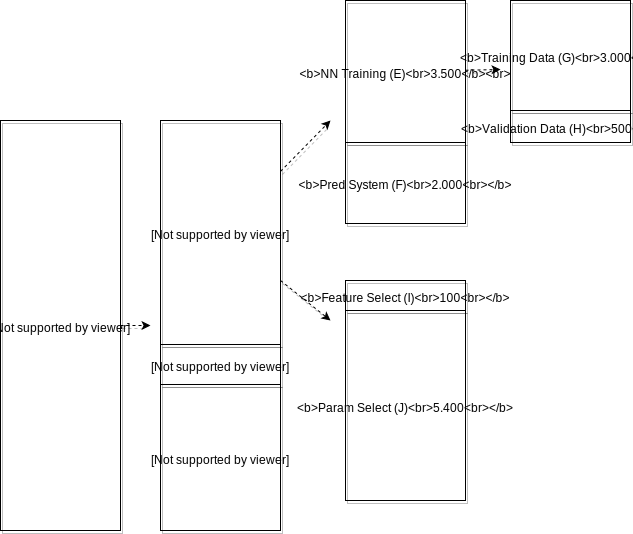
\includegraphics[width=.8\textwidth]{./pictures/data/Data.png}
    \caption{Shows how we have split the dataset we are given. The splits are
        performed on the number of authors in each set. That means that all of
        an authors texts are contained in the same dataset. In particular that
        means that the test dataset contains completely unseen authors that has
        not been used in any training/hyper-parameter selection.}
    \label{fig:data_split}
\end{figure}

\begin{itemize}

    \item[- (A).]

        The entire set of extracted data. This consists of text written by,
        10.058 different danish high school students, spanning different schools
        throughout the country.

    \item[- (B).]

        Consisting of the texts written by 5.500 different authors, this set
        if used in the training process for the \gls{NN}s where it is used for
        training/validation and the prediction system. It is also used for the
        baseline methods, where this entire set is used as the corpus.

    \item[- (C).]

        Being untouched throughout the training process, this set is used for
        unbiased validation, and selection of networks to be used on the test
        set (D). Contrary to the training set (B), this is only used for the
        final selection of our best models during the training process.

    \item[- (D).]

        The test set, which as the name implies, is used to test the performance
        of our final models.

    \item[- (E).]

        As mentioned (B) is used for training both the baselines and the
        \gls{NN}s. In both circumstances, and different split of (B) is
        performed. (E) is the data used for the actual training of the
        \gls{NN}s.

    \item[- (F).]

        This set is used as the basis of the prediction system described in the
        earlier sections of this paper.

    \item[- (G).]

        The training data which is given to our \gls{NN}s.

    \item[- (H).]

        A separate validation set, where no authors overlap with (H), which is
        used to determine the accuracy of our the model on an independent set
        of authors during training. This allows us to stop the training when we
        reach the desired generalization and accuracy.

    \item[- (I).]

        This is an alternate split of (B), used on the baseline methods together
        with set (J). It is used perform the feature selection for both the SVM
        and the Extended Delta method. The specifics of this process will be
        described in Section \ref{subsec:baseline}.

    \item[- (J).]

        This set is used to tune the baseline methods. (J) is used to determine
        the best hyper-parameters for the baseline methods. This would be K and
        p in the case of the Extended Delta Method, and C and Gamma for the SVM.
        Like with (I), the specifics of this parameter selection will be covered
        in Section \ref{subsec:baseline}.

\end{itemize}

The training set (B), consists of a total of 73311 texts written in the same
class, split over the 5.500 authors, from different schools. Each authors has
written in average 13 texts, with the standard deviation being 4.2. We initially
removed the first 200 characters of each text, as the beginning of each text
contains a lot of authorship identifying information, such as name, school, and
specifics class. The removal of these characters also make sure that no garbage
texts are included. The texts vary a lot in both structure and length, spanning
from poems to essays. It is for this reason that this sets character count has
a standard deviation of 4133 even though the average character count of 5516.
The full statistics of the training set (B) can be seen in the appendix, Section
\ref{sec:B_stats}.

Due this to this disparity in terms of the contents of the data, some
constraints had to be applied to the data. The reason for this is ,in most
cases, that the non-existence of the constraints would result in either some
computational inefficiency accompanied by a minor increase in data-quality, or
simply just a computational impossibility such as a single text consuming all
memory causing our models to crash. Another purpose of these constraints is to
make the data-set generalize better by removing the outliers.

As can be seen in the statistics in Section \ref{sec:B_stats}, the text
containing the smallest consists of 0 characters, and does obviously not
contain any valuable information. In addition to the 200 characters we removed
initially, we also removed texts that have below 200 characters left after the
removal, as they do not provide enough information about that specific author,
and would work properly with our baseline methods due to the size.
The application of this constraint, resulted in 1.823 of the 73.311 texts
being removed. After which we applied a upper constraint, in terms of the total
number of characters. The reason for this, was a mentioned earlier, that there
are some texts eating up all the available memory, such as the largest text in
(B), which consists of 338.315 characters. We found that limiting the number of
characters to 30.000 gave good results, by removing the crash-inducing texts,
without affecting the overall data-quality too much, as this only removed 119
texts from (B).

Since we also perform some sentence level networks as well, we also chose to
limit the max number of sentences, for the same reason as with the characters.
The text with the largest amount of sentences, contains 4401 sentences. With
an average sentence count of 49 and a standard deviation of 39, this text is
obviously an outlier, and doesn't generalize the data set very well. A such we
impose a upper limit of 500 sentences per text, which removes another 26 texts
from (B).

The last constraint regards the unique characters in each text. Look at the
stats we can see that there is a text containing 219 unique characters, greatly
exceeding the average of 57. A unique character count like this, implies that a
non-danish alphabet might have been used, and for that reason texts like these
do not add to the generalization we strive towards. This is combatted creating a
list of characters based on the data used for training, each character in this
list is mapped to a replacement character if ever encountered in either the
training or the validation set. The characters are placed in this list if they
occur with a frequency smaller than $10^{-5}$. This threshold was determined
by looking at the danish characters Æ,Ø and Å. In the set (B) they have
a frequency just above $10^{-5}$. We want these included, as we hypothesize
that they generalize danish student well. Additionally we can see in Figure
\ref{fig:character_frequencies}, along with the other thresholds, that after
the character frequency threshold, the overall of frequency of the specific
characters drops dramatically.

After applying all of the constraints, and taking into account
overlap between them, 1.944 texts were removed from the total 73.311 in (B),
which is a negligible amount compared to the computational and generalization
advantages it includes.
In the end this leaves set (B) with 71.367 texts.

The aforementioned constraints were not all applied to entirety (A) in the same
manner. Both (C) and (D) are used in a testing context, for that reason removing
the first 200 characters wont make sense as we only did that to prevent the
training process in latching on to author specific meta-data in the text. We
still apply the lower constraint of 200, as this system was intended for usage
of the large SRP assignment the students make at the end of their last year,
this this constraints scrubs away potential garbage texts. The upper limit
is removed, as this was only a step to prevent our methods from crashing. By
applying the methods on a students assignment in a singular fashion rather than
a batch one, we will not have the same problem.

\begin{figure}[htb]
    \begin{minipage}{.5\linewidth}
        \centering
        \subfloat[]{\label{main:a}\includegraphics[scale=.5]{./pictures/data/Frequencies.png}}
    \end{minipage}%
    \begin{minipage}{.5\linewidth}
        \centering
        \subfloat[]{\label{main:b}\includegraphics[scale=.5]{./pictures/data/SentenceCount.png}}
    \end{minipage}\par\medskip
    \centering
    \subfloat[]{\label{main:c}\includegraphics[scale=.5]{./pictures/data/CharacterCount.png}}

    \caption{The different thresholds applied to the during preprocessing.}
    \label{fig:character_frequencies}
\end{figure}

All of the neural networks we train are Siamese Neural Networks. They all
work by comparing two texts at a time. We therefore had to generate problem
instances that contained two texts from either the same or different authors and
a class that reflected that. For each author $\alpha$ in the training dataset
$G$ we generate all possible combinations of two of the texts in $T_\alpha$
as positive samples. We also generate the same number of negative samples by
taking a random text in $T_\alpha$ and a random text in $\overline{T_\alpha}$.
That means that in total the number of problems we generate for each author
is $ 2\frac{\left|T_\alpha\right|!}{2!(\left|T_\alpha\right|-2)!} = 2 \cdot
(\left|T_\alpha\right| - 0) \cdot (\left|T_\alpha\right| - 1) $. The neural
networks are trained on these problem instances. We generate problems in the
same way for the network training validation dataset $H$.

    \FloatBarrier

    \section{Experiments} \label{sec:experiments}


\subsection{Baseline Methods}

In this section we will go through the experiments performed in order to get
our baseline results. While many different features can be used when performing
\gls{NLP}, we chose the same features, as was used in \cite{US}, since they
span several several of the different linguistic layers. The linguistic layers
are different areas which all serve to describe a certain text. An example this
could be the character level layer, which as the name implies, focuses on the
individual characters used in a specific text. Other examples of this, could the
sentence layer, that focuses on the sentences of the text, and the meta layer,
that focuses on things such as publishing/delivery date, and file format. The
features available to pick from in this case are:

\begin{itemize}
    \item Word-N-grams,
    \item Character-N-grams,
    \item Word Frequencies (word-1-grams),
    \item \gls{POS}-tag-N-grams, and
    \item Special-Character-N-grams,
\end{itemize}

Where an N-gram describes the combinations of sequential elements of size n. In
the case where that element is characters, and n is 3, the string "hello" would
produce the character-3-grams "hel", "ell" and "llo". This also means that a
feature such as word frequencies can be considered word-1-grams.

For all of these experiments a Danish third party corpus, provided by
\texttt{NLTK}\footnote{\url{http://www.nltk.org/index.html}}, was used as the
basis for all the feature extraction, as was done in \cite{US} as well. This
corpus consists of 22,476 sentences, and 563,358 words.

The actual implementation of both the \gls{SVM} and the Extended Delta method,
very closely resembles the implementation used in \cite{US}. There is however
a very big difference, with the actual application of the delta method.
Contrary to the scenario in \cite{US}, where PAN data was used, there isn't an
instance where we only have 1 text per author. As such the original version
of the delta method can be used. This is where, when given a new text $x$
supposedly written by an author $\alpha \in \mathcal{A}$, his texts $T_\alpha$
are extracted, and so is a set of texts no written by him $\overline{T}_alpha$
where $|\overline{T}_\alpha| = |T_\alpha|$. The text, along with a negative
sample text $z$, we know now to be written by $\alpha$ is given to a \gls{KNN}
classifier, which determine if $x \in T_\alpha$ and $z \in \overline{T}_alpha$.

\subsubsection{Feature Selection}

A large part of the experiments performed when applying the extended delta and
\gls{SVM} method was parameter tuning. Neither method does any quality analysis
of the feature they are applied on, as other methods such as the random forest
does. This means that they are susceptible to noisy feature, and as a result
would most likely benefit from us selecting the features for them.

Before starting any kind of feature selection or hyper-parameter tuning,
we split the training data up into training and validation, with a 
80/20 respective split. All the work described from this point on,
was done on the 80\% training.

Contrary to our previous work made in \cite{US}, this process wont
consist of trying out some random selection of features, but rather
a more systematic approach was used. 

However, before starting to do that, a feature set was to be created
first. In order for us to find the very best set of features, we wanted
to create a very large feature set, so as to increase our search space.
The corpus used had the following quantities of the different features.

\begin{itemize}
    \item Word-2-grams - 188,472
    \item Character-2-grams - 2,178
    \item Word Frequencies - 27,535
    \item \gls{POS}-tag-2-grams - 219
    \item Special-character-2-grams - 524
\end{itemize}

The quantities here are of course very large due to the size of the corpus,
and will continue to rise as N increases. Rather than extracting all
of those feature from our texts, we chose to focus on the most N-grams
with highest frequency, as we would reach a point where a specific N-gram
determined to be in the corpus, would be unique that same corpus, making it
irrelevant for new texts, not associated with the corpus.

Using the quantities listed above as inspiration, a feature set of around 5000
features was produced, containing

\begin{itemize}
    \item The 500 most frequent words,
    \item The 500 most frequent word-N-grams for $N \in \{2,3,4\}$,
    \item The 300 most frequent character-N-grams for $N \in \{2,...,10\}$,
    \item The 50 most frequent \gls{POS}-tag-N-grams for $N \in \{3,4\}$, and
    \item The 50 most frequent special-character-N-grams for $N \in \{2,3,4\}$.
\end{itemize}

The selection the quantities, bases on the number available in the corpus,
as listed earlier. As the for the N in the N-grams, \cite{aalykke2016} found
out that char-8-grams worked very well in his case, which is why N goes all
the way to 10 in the case of char-N-grams . Looking at the results
from \cite{US}, Word-N-grams mostly stopped occurring in texts when getting
to 4-grams, when looking at the result from \cite{US}. A similar thing
could be seen with the special-character-N-grams, where an increase in N,
wouldn't contribute anything. \gls{POS}-tag-N-grams were a really big burden
computationally, as such a reduction in possible N-values, had to be made.

These features were extracted from the same data-set described earlier in
section \ref{sec:data}. However it wasn't beholden to the same exact limits to
character and unique characters. In the case of the upper limit the lack of
memory wasn't nearly as severe as in the case of our \gls{NN}s. As for the lower
limit, and natural boundary would occur throughout the extraction process.
If a file did not have 500 unique words for example, the extraction
of the 500 most frequent words would cause an error, resulting in that
text being ignored.
The distribution of the texts over authors in this data-set isn't
very evenly spread. As such, the random selection of random opposing
authors has a certain amount of bias towards the authors with a large
amount of texts compared to the test.

Having the features, we could start doing our feature selection. This whole
process proved very expensive computationally. Having to check every permutation
of 5000 features, simply wasn't feasible. It was for that reason we opted for
a greedy algorithm instead.

This greedy algorithm works as described by \cite{kanDeng}, which is a simple
forward feature selection. Having out previously created feature set, we loop
through each single feature, validating its' accuracy when applied to each
$\alpha \in \mathcal{A}$. As eluded to earlier, this consists of fetching
$T_{\alpha}$ and a set $\overline{T}_{\alpha}$, where $|\overline{T}_\alpha| =
|T_\alpha|$. Using this set of positive and negative cases, we make use k-fold
cross validation to determine the performance of the feature for that author.
This is done for all authors, and when averaged we have the performance of
that single feature. This process is then repeated for all features. The best
performing feature is then added to out candidate set of features. The next
iteration we loop through all the feature again, but we validate against each
feature in combination with the already selected features. This process is
repeated until a set number of features are selected. At this point we determine
at which point we had the best candidate set, and use that hence fourth.

Even this greedy approach proved to be very time consuming. As such, we only did
as described and found the best features, but left out the hyper-parameters C,
and $\gamma$ for the SVM, and K and the distance metric for the extended delta
method. These hyper-parameters were also selected through a separate process
which will be described in a later section.

The cross validation used differs from each method. The SVM uses normal 3 fold
cross validation. This however was not the case for the extended delta method.
The reason for this was that there was a scenario where an unlucky split of
folds would cause a lot of error. A generic example of this would be if we
had the 2 class training set consisting of 6 value, evenly split between the
2 classes. In the case where we split those 6 values into 3 folds, there is a
chance that a fold contains two value of the same class, which means that if $K
= 3$ in our case, both of those wont ever be able to classified correctly as
there is only 1 of that class in the training set. As such, stratified K fold
cross validation is used instead, as it uphold the class distribution in its'
folds. Leave one out cross validation would of course also work in the case of
both out methods, but we were limited by the computation time, and for that
reason we opted for K folds instead.

For both the \gls{SVM} and Extended Delta method, we ran this algorithm
until 250 features were selected. Computation time was still and issue, so
additionally we only made use of 5\% of the total number of authors. The SVM
performed its' feature selection using the default RBF kernel, a C with value 1,
and $\gamma = \frac{1}{\text{n\_features}}$. Due to some authors having below
3 texts, the default K value of \gls{KNN}s K parameter was set to 3 for the
feature selection.

The results of both the SVM and the Extended Delta method feature selection
can be seen in figure \ref{fig:fs_results}. (DISCLAIMER: Extended Delta is
erroneous)

The SVM ended up peaking having selected 225 features, with an accuracy of
0.649. The features whose addition causes the largest accuracy values can be
seen in \ref{table:svm_feature}

TODO: Extended Delta Results

\begin{figure}
\centering
\includegraphics[scale=0.8]{./pictures/experiments/baselines/FeatureSelect.png}
\caption{The process of the greedy feature selection of the SVM and the Extended Delta Method}
\label{fig:fs_results}
\end{figure}


\subsection{Hyper Parameter Selection}

As mentioned in the previous section, due to computational time, we were unable
to do the hyper parameter selection parallel with the feature selection. 
For that reason we chose to split it up, selecting our features first, and the 
fine tuning our parameters based on those selected features.

This means that our implementation very closely mimics the one used in the
previous example. On both cases we start out with two lists of possible hyper
parameter values:

\begin{align}
SVM&:
		\begin{array}{lr}
        C=\{10^{-2}, 10^0, 10^2, 10^4, 10^6, 10^8, 10^{10}\}\\
        \gamma=\{10^{-7}, 10^{-5}, 10^{-3}, 10^{-1}, 10^{1}, 10^3, 10^5\}
        \end{array}\\
\text{Extended Delta}&:
		\begin{array}{lr}
        p=\{1,2,3,4,5\}\\
        K=\{1,2,3,4,5,6,7,8,9,10,11,12,13,14,15\}
        \end{array}
\end{align}

The one parameter yet to be explained i $p$, which refers to the p in the
minkowski distance.

$$
D(X,Y) = \left(\sum_{i = 1}^n |x_i - y_i|^p\right)^{1/p}
$$

Where $p=1$ and $p=2$ is the manhattan and eucledian distance respective.

We perform a grid search over all these parameters. For each variation of the
hyper parameters we average the performance of the method over all unique
authors in the training set, in a manner very similar to the feature selection.
A key difference is that rather than using 3 fold cross validation, we now use
leave one out cross validation. We aren't performing nearly as many iterations
this time around, which is why this change was made. In this case, we loop
over all unique authors one time for each combination of hyper parameter, the
number of which dwarfs the amount in the feature selection. The accuracy of each
parameter configuration can be seen in figure TODO:ref, and figure TODO: ref.

After the best parameters were found, we apply the methods to the 20\% we set
aside for validation originally. This resulted in the SVM getting an accuracy of
0.713 with its best parameters being $C=100.0$ and $\gamma=1000$.

TODO: Extended Delta Results

%\subsubsection{Author Specific SVM}
%
%The author specific SVM is a authorship verification method that learns from
%hand crafted features. Similar to the Extended Delta method we perform a feature
%search in a large set of features to find the optimal features for the SVM. To
%evaluate different feature sets and different hyperparameters we use the
%algorithm shown in Figure \ref{fig:svm_evaluation_algorithm}. The algorithm
%computes the average accuracy of the SVM via leave one out cross validation. For
%each author it takes a set of texts written by that author and a set of texts of
%similar size written by another author. Then it successively leaves out one of
%the texts, train an SVM on the rest and then use that SVM to predict the class
%of the text that was left out. The score is then the average accuracy of that
%prediction.
%
%\begin{figure}
%    \begin{algorithm}[H]
%        \KwData{$A$ a set of authors, $F$ a set of features, $C$ SVM
%        hyperparameter, $\gamma$ SVM hyperparamter}
%        Let $S = \emptyset$\;
%        \For {$\alpha \in A$} {
%            Let $T_k = T(\alpha)$\;
%            Let $T_u = \{
%                x_i\ |\ x_i \in \mathcal{U}\left(
%                    \overline{T}(\alpha)
%                \right), 1 \leq i \leq \left| T_k \right|
%            \}$\;
%            \label{line:draw_opposition}
%            Let $F_k = \{ f(t, F)\ |\ t \in T_k\}$\;
%            \label{line:feature_extract_1}
%            Let $F_u = \{ f(t, F)\ |\ t \in T_u\}$\;
%            \label{line:feature_extract_2}
%            \For {$x \in F_k \cup F_u$} {
%                Let $m = SVM(F_k \setminus x, F_u \setminus x, C, \gamma)$\;
%                \uIf {$m(x) = a(x)$} {
%                    Let $S = S \cup \{1\}$\;
%                } \uElse {
%                    Let $S = S \cup \{0\}$\;
%                }
%            }
%        }
%        \Return {$\mu(S)$}
%        \caption{SVM evaluation}
%    \end{algorithm}
%    \caption{Algorithm to evaluate an SVM on a set of authors. The algorithm is
%        given a set of authors $A$ to evaluate over, a set of features $F$ to
%        use and the hyperparameters for the SVM. On Line
%        \ref{line:draw_opposition} $\mathcal{U}$ denotes the uniform
%        distribution and $T_u$ is a set of texts of the same size as $T_k$ where
%        each text in the set is written by a different author than $\alpha$. On
%        Line \ref{line:feature_extract_1} and Line \ref{line:feature_extract_2}
%        $f$ denotes a function that computes the features $F$ of the text $t$.
%        The algorithm computes the average accuracy of an SVM with the paramters
%        given over all authors given.}
%    \label{fig:svm_evaluation_algorithm}
%\end{figure}
%
%The search in a set of features $F$ are performed by starting with an
%empty set of features $FC$. Then in each iteration we add a single
%$f \in F$ to $FC$ and evaluate the SVM with the algorithm in Figure
%\ref{fig:svm_evaluation_algorithm}. At the end we add only the single feature
%that gives the best performance in the evaluation algorithm and repeat again
%with the rest of the features. The feature set we search in are the same feature
%set as the feature set used in the Extended Delta Method but without limiting
%the number of texts per authors. The search are performed on only 100 random
%authors in the set as it otherwise takes to long. The feature search is done
%with fixed SVM hyperparameters which we tune afterwards. The hyperparameters
%used during the search was $C = 100$ and $\gamma = 1000$, and using the default
%rbg kernel. The feature search surprisingly found only 6 features before no
%features could improve the result further. The specific features were the
%character-2-gram " -", the character-3-gram ", o", the character-4-gram ", at",
%the character-4-gram ", so", the character-6-gram ", der " and the word-1-gram
%"giver". Most of the features seem to look at what authors are writing
%immediately following commas. We found the optimal hyper parameters for the SVM
%by splitting the dataset in two parts. 80\% of the authors went in the training
%part and 20\% of the authors went in the validation part. Then for each author
%in the training dataset we varied $C \in (10^{-2}, 10^0, \dots, 10^{10})$ and
%$\gamma \in (10^{-9}, 10^{-7}, \dots, 10^3)$ and evaluated an SVM using the
%algorithm in Figure \ref{fig:svm_evaluation_algorithm} with the fixed feature
%set for each combination of hyperparameters. After that we took a majority
%vote between the authors chosen hyperparameters and chose that as the final
%hyperparameters. The final hyperparameters were $C = 100$ and $\gamma = 1000$.
%We then evaluated our chosen parameters both feature set and hyperparameters on
%the validation set. We obtained an accuracy of 0.62980.
%
%Since we were surprised that only 6 features were used we also tried to take a
%feature set of the 50 most frequent features in each category. We again ran the
%search for hyperparameters. This time we found that $C = 100$ and $\gamma = 10$
%worked the best. We obtained an accuracy of 0.69552. So we were able to obtain a
%higher accuracy by arbitrarily choosing the 50 most frequent features instead of
%doing a structured search.
%
%TODO: Try using all features.


\subsection{Deep Learning}

The main attraction of our authorship verification task, is the implementation
and testing of different \gls{NN}. In the following sections we will go through
the different iterations of networks we have produced. A glossary of the
different layers used can be seen in figure \ref{glossary}. Throughout out
experiments, we used a 0.5 threshold for classification.

\begin{landscape}
    \begin{table}
        \centering
        \caption{Glossary used when performing experiments, and creating their
            associated models.\cite{chollet2015keras}}
        \label{glossary}
        \begin{tabular}{|L{3cm}|L{9cm}|L{11cm}|}
            \hline
            % TODO: Should center header.
            \textbf{Layer}                                                     &
            \textbf{Description}                                               &
            \textbf{Actively Used Parameters}                                 \\
            \hline

            Input                                                              &
            Serves as the entrypoint of the network, by receiving a set of
            texts and feeding it trough the network.                           &
            \begin{minipage}[t]{\linewidth}
            \begin{compactdesc}
                \item[Shape] The dimensions of each sample give to the input.
            \end{compactdesc}
            \end{minipage}                                                    \\
            \hline

            Embedding                                                          &
            Taking in an encoded sample, it produces a dense vector
            representation for each different. More details can be found in
            Section \ref{subsubsec:layers}.                                    &
            \begin{minipage}[t]{\linewidth}
            \begin{compactdesc}
                \item[Input Dim] Size of vocabulary.
                \item[Output Dim] Size of vector used to represent embedding.
            \end{compactdesc}
            \end{minipage}                                                    \\
            \hline

            Convolutional                                                      &
            Applies convolution to the data it recieves according to the
            decription, found in Section \ref{subsubsec:layers}.               &
            \begin{minipage}[t]{\linewidth}
            \begin{compactdesc}
                \item[Filters] Dimensionality of the output, ie. number of
                    filter from the convolution.
                \item[Kernel Size] Integer or list describing size of
                    convolution window.
                \item[Strides] Stride length of the convolutional window.
                \item[Activation] The activation function to be applied after
                    the convolution.
            \end{compactdesc}
            \end{minipage}                                                    \\
            \hline

            Global Max Pooling                                                 &
            Extracts the maximum value from each of the provided data          &
            No parameters.                                                    \\
            \hline

            Concatenation                                                      &
            As the name suggests, this layers simply concatenates the data it
            receives from different layers                                     &
            No parameters.                                                    \\
            \hline

            Merge                                                              &
            Merges its inputs, using a specified function to generate a single
            output.                                                            &
            \begin{minipage}[t]{\linewidth}
            \begin{compactdesc}
                \item[Function] The function used to merge the recieved data.
            \end{compactdesc}
            \end{minipage}                                                    \\
            \hline

            Dense                                                              &
            A simple fully connected layer, taking in data and applying the
            function described in Section \ref{sec:neurons}.                   &
            \begin{minipage}[t]{\linewidth}
            \begin{compactdesc}
                \item[Units] Number of neurons in in the layer.
                \item[Activation] The activation function to be applied.
            \end{compactdesc}
            \end{minipage}                                                    \\
            \hline

            Dropout                                                            &
            Drops a fraction it receives, with the goal of preventing
            overfitting.                                                       &
            \begin{minipage}[t]{\linewidth}
            \begin{compactdesc}
                \item[Rate] The fraction of data it receives dropped.
            \end{compactdesc}
            \end{minipage}                                                    \\
            \hline

            Lambda                                                             &
            Applies a specified function to the input it receives              &
            \begin{minipage}[t]{\linewidth}
            \begin{compactdesc}
                \item[Function] The function applied.
            \end{compactdesc}
            \end{minipage}                                                    \\
            \hline

            Reshape                                                            &
            Reshapes the data it receives.                                     &
            \begin{minipage}[t]{\linewidth}
            \begin{compactdesc}
                \item[Dim] Dimensionality to reshape to.
            \end{compactdesc}
            \end{minipage}                                                    \\
            \hline

            GRU                                                                &
            A gated recurrent unit is applied to the data according to the
            description found in Section \ref{subsubsec:layers}.               &
            \begin{minipage}[t]{\linewidth}
            \begin{compactdesc}
                \item[Unit] Number of neurons in the layer.
            \end{compactdesc}
            \end{minipage}                                                    \\
            \hline

            LSTM                                                               &
            A Long Short-Term Memory layer, which works according to the
            description in Section \ref{subsubsec:layers} is applied to the
            given data.                                                        &
            \begin{minipage}[t]{\linewidth}
            \begin{compactdesc}
                \item[Unit] Number of neurons in the layer.
            \end{compactdesc}
            \end{minipage}                                                    \\
            \hline
        \end{tabular}
    \end{table}
\end{landscape}

\subsubsection{Siamese Neural Network - Iteration 1}

The network we used to try and solve the problem is shown in Figure
\ref{fig:network_1}. The Siamese part of the network is the Convolutional
Layer. We used 1000 filters of size 10. That means that 1000 different features
are supposed to be learned by the network and each feature can use a local
context of 10 characters to extract a feature. After the convolution we have a
max-over-time pooling layer. The layer takes the maximum value of each feature
such that we have 1000 features from each text. We then have a normal dense
neural network on top of that which are given the features of both texts. The
dense network is then supposed to learn how to compare the features from the two
texts. We have 1 dense hidden layer each with 500 neurons. At the end we have
a output layer with two outputs. The activation function for all layers except
the last one is the rectified linear unit and the activation function of the
last layer is the softmax function. The output of the network is a probability
distribution over the two classes.

The input to the network first goes through an embedding layer. The embedding
layer transforms integers into dense vectors of floating point numbers. The
embedding layer functions as a lookup table such that each integer is mapped
to the same dense vector. The embedding is trainable meaning that better
embeddings will be learned while the network is training.

\begin{figure}[htb]
    \centering
    \includegraphics[width=0.6\textwidth]{./pictures/experiments/network1.png}
    \caption{Illustrate the structure of our first Siamese Neural Network
        Architecture.}
    \label{fig:network_1}
\end{figure}

The network obtained a validation accuracy of 0.68684. We have shown both the
training and validation accuracies in the different epochs in Figure
\ref{fig:network1_accuracies}. In that plot we can see that the network very
quickly overfits the training data and no longer learns anything general.

\begin{figure}[htb]
    \centering
    \includegraphics[width=0.5\textwidth]{./pictures/experiments/network_1_accuracies.png}
    \caption{Training and validation accuracies for the iteration 1 network in
        the different epochs of the networks execution.}
    \label{fig:network1_accuracies}
\end{figure}


\subsubsection{Siamese Neural Network - Iteration 2}

% TODO: Illustrate how dropout corresponds to training different subnetworks in
% each iteration.

In our last network we observed that the network after a few number of epochs
overfitted on the training dataset. The validation accuracy quickly began
stalling as the training accuracy went to 100\%. We therefore focused our
second network architecture on limiting overfitting. We added a dropout layer
before the output layer. The layer prevents overfitting by making sure that
the network cannot rely on the output of all neurons during training. This
unpredictability makes it harder for the network to learn specific quirks of
the training dataset since small quirks will only be picked up by a small
amount of neurons while larger trends will be represented by a larger set
of neurons. \cite{JMLR:v15:srivastava14a} investigated the use of dropout
layers in different problem settings. They found that dropout layers reduced
overfitting in all problems they looked at. In particular they found that
document classification which is similar to what we are doing were also
improved. The main drawback of a dropout layer is that it increase the run time
of training the networks (\cite{JMLR:v15:srivastava14a}).

In iteration 1 the function we used to merge features from the known and unknown
text together were a concatenation. If we let the extracted features of the
known text be $K_i$ and the extracted features of the unknown text be $U_i$ then
$K_0$ and $U_0$ correspond to the same feature extracted from the two texts. The
concatenation merge function would then produce,

\begin{equation}
    merge(K, U) \rightarrow \left(
        K_0, K_1, \dots, K_n, U_0, U_1, \dots, U_n
    \right)^T.
\end{equation}

That means that the neural network would have to figure out by itself that input
$0$ were related in particular to input $n + 1$. To save the network that task
we also replaced the merging function to the absolute difference of the feature
vectors. That means that our merge function became,

\begin{equation}
    merge(K, U) \rightarrow \left(
        (|K_0 - U_0|), (|K_1 - U_1|), \dots, (|K_n - U_n|)
    \right)^T.
\end{equation}

So the network no longer has to learn arbitrary indexes. Instead it can learn
which features is important for authorship verification and learn thresholds for
when each feature is important. With the new merging we will have a large number
whenever the two features are far apart and a small number whenever they are
close to each other.

We changed the convolutional filters we used from 1000 convolutional filters of
size 10 to 500 convolutional filters of size 4 and 500 convolutional filters of
size 8. The idea was that the filters could learn different features where some
of the features would consist of a large number of characters and other of the
features would consist of a small number of characters. The architecture of our
network from iteration 2 is shown in Figure \ref{fig:network_2}.

\begin{figure}
    \centering
    \includegraphics[width=\textwidth]{./pictures/experiments/network2.png}
    \caption{Illustrate the structure of our second Siamese Neural Network
        Architecture.}
    \label{fig:network_2}
\end{figure}

We also added more dense layers to the model. A plot of the
training and validation accuracies per epoch can be seen in Figure
\ref{fig:network2_accuracies}.

\begin{figure}
    \centering
    \includegraphics[width=0.5\textwidth]{./pictures/experiments/network_2_accuracies.png}
    \caption{Shows the training and validation accuracies on the second
        network.}
    \label{fig:network2_accuracies}
\end{figure}

The maximum validation accuracy obtained were 0.74464 in epoch 12.


\subsubsection{Siamese Neural Network - Iteration 3}

In iteration 2 we observed that the network seemed to learn everything in the
first epoch and didn't improve much after that. We also observed that the
accuracy improved compared to the first network. We therefore wanted to try a
larger network which would be able to hopefully learn more and obtain a higher
accuracy than our first two networks.

We both tried adding more convolutions and adding more dense layers. Our third
network use 700 convolutions of size 8 (currently drawn confusingly) and 500
convolutions of size 4. The network then contains 4 dense layers all with 500
hidden neurons with \gls{ReLu} activation function. Then a dropout layer with
30\% dropout and finally the output layer with 2 neurons and a softmax
activation function. The function we use to combine the features from the two
texts are still the absolute difference as that seemed to work fine for the
previous network. We have shown the structure of the third network in Figure
\ref{fig:network3}.

\begin{figure}
    \centering
    \includegraphics[width=\textwidth]{./pictures/experiments/network3/network3.png}
    \caption{Illustrate the structure of our third Siamese Neural Network.
        Weights are shared by the embedding layers and the convolutional
        layers.}
    \label{fig:network3}
\end{figure}

Our third network were able to obtain an accuracy of 0.83612. We have shown the
training and validation accuracies in Figure \ref{fig:network_3_accuracies}. We
can see that the network quickly improve to about 80\% accuracy and after that
not much happens.

\begin{figure}
    \centering
    \includegraphics[width=0.5\textwidth]{./pictures/experiments/network_3_accuracies.png}
    \caption{Shows the training and validation accuracies over the epochs of
        training on the third network.}
    \label{fig:network_3_accuracies}
\end{figure}

To get an idea of which features the network were looking at we looked at the
output of the convolutional layers. After the convolutional layers we have a
max-over-time pool so we know that higher values are important. We could then
take a text, feed it to the network, find the index of the maximum output of
the convolutional layers and then show the text snipped (char-N-gram) that
produced that high value. We then did that for all the texts in the dataset. The
first filter in the network for example yielded many short strings ending with 3
newlines. Some examples of these are,

\begin{lstlisting}[gobble=4]
    'adsen\n\n\n'
    'ndsen\n\n\n'
    'umeer\n\n\n'
    'endte\n\n\n'
    'ingen\n\n\n'
    'ehren\n\n\n'
    'elsen\n\n\n'
    'ommer\n\n\n'
    'Ruter\n\n\n'
    'ummer\n\n\n'
    'ersen\n\n\n'
    'ansen\n\n\n'
    'heden\n\n\n'
    'ensen\n\n\n'
    'arsen\n\n\n'
    'orten\n\n\n'
    'ulsen\n\n\n'
    'orgen\n\n\n'
\end{lstlisting}

Many of those short string looks like the ending of common Danish
names followed by three newlines. Here are some examples of the
names taken from a list of the 100 most frequent surnames in Denmark
\footnote{http://www.mydanishroots.com/surnames-meaning-and-origin/the-100-most-
common-surnames-in-denmark.html},

\begin{description}
    \item[adsen:] Madsen.
    \item[ndsen:] Svendsen, Frandsen.
    \item[elsen:] Nielsen, Mikkelsen.
    \item[ersen:] Pedersen, Andersen, Petersen, Iversen, Jespersen.
    \item[ansen:] Hansen, Christiansen, Johansen, Kristiansen.
    \item[ensen:] Jensen, Christensen, S\o rensen, J\o rgensen, Kristensen,
        Mortensen, Mogensen.
    \item[arsen:] Larsen.
    \item[ulsen:] Poulsen.
\end{description}

The network therefore seems to have learned that a name followed by whitespace
are an important feature when determining the authorship of a text. Clearly when
a student buy an assignment from a ghost writer the text will contain the
students own name. Therefore these features are counter productive since the
network learns that as a result of how we have created the training dataset
where each text has the correct authors name in it.


\subsubsection{Siamese Neural Network - Iteration 4}

In this iteration we trained the third network again but now using a dataset
where names were substituted by empty strings. We wanted to see how well the
network would perform when it was not able to use peoples names as a feature.
A graph of the training and validation accuracies can be seen in Figure
\ref{fig:network_4_accuracies}. The best validation result we found was in epoch
22 with an accuracy of 0.79843. That means that we lost about 4\% accuracy now
that we can no longer look at peoples names.

\begin{figure}
    \centering
    \includegraphics[width=0.5\textwidth]{./pictures/experiments/network_4_accuracies.png}
    \caption{Shows the training and validation accuracies over the epochs of
        training on the fourth iteration of the network.}
    \label{fig:network_4_accuracies}
\end{figure}

We wanted to verify whether or not the network still looked at the names of the
authors. It is not possible for us to look at all 1200 filters but we looked
at a couple and did not find any that looked like they were looking at names.
However we did find that the network now seems to be looking at which class
the student is in. The classes in Danish schools are typically written as 1.p,
1.q, 2.p, 2,q, etc. and we found that one of the convolutional 4 filters were
looking at character sequences such as those. We have generated a couple of
tables that shows what the network is now looking at. We generated the tables by
taking the first 50 texts from the dataset and extracting the maximum value of a
particular filter from each text. That gives a single string of the convolution
size from each text and a number which is higher the more important that string
is. We then sorted the extractions by the importance score. The result of a
couple of the filters are shown in Figures \ref{fig:features_convolution_8_1},
\ref{fig:features_convolution_8_5}, \ref{fig:features_convolution_8_100} and
\ref{fig:features_convolution_4_100}. The first figure looks at whether or not
authors use the phrase "s\aa\ at" (such that). Inexperienced Danish writers will
often use the phrase which is considered grammatically incorrect in most Danish
sentences. Therefore the network seems to have learned that some writers use
"s\aa\ at" while others don't and that it is an important phrase when verifying
authorship. The second figure seems to look at whether or not an authors uses
the phrase "meget" (most). Some authors apparently often describe things using
"meget" while others do not. The third figure shows that the network looks at
which authors use the phrase "at de" or "at der" ("that they" or "that there").
The fourth filter is the one that seems to look at which class a student is in.
In our constructed dataset the class of a student will always be a good feature
since we don't have any actual ghost writers. However a ghost writer would write
the correct class of the student on their submission. Therefore we don't want
the network to learn that particular feature.

Our main problem is that the networks keep using metadata from the texts to
make the predictions. The metadata will always match even though a ghost writer
has written the assignment. It is probably not possible for us to remove all
metadata from all texts. Even though names are supposed to have been removed
the dataset still contains a couple of them and there is so many different ways
of writing the class of a student that it is not feasible for us to remove
all of them. The metadata will typically occur in the beginning of the text
and sometimes throughout the text in headers. When training a neural network
on images it is normal practice to rotate, shift, shear and zoom the images
randomly during training. The shifting of the images produces new images where
part of the image is no longer part of the training set. In each epoch the
image is shifted a different amount in different directions and the network can
therefore learn to recognise objects even though part of the image is not there.
We wanted to do something similar for the texts we are training on. At the
moment the network relies on finding metadata in the text. That is only possible
when it is given the whole text since metadata will only occur in parts of the
text. We therefore want to try to only give part of the texts to the network
during training. We can do that by replacing some random part of the input text
with a special value during training. For example each time a text is used
during training we might replace 50\% of it with a special garbage character.
Therefore the network will no longer be able to rely on finding metadata about
the text since the metadata will not always be present.

Another problem our current networks has is that each filter extract
only a single value from a text. For example the filter shown in Figure
\ref{fig:features_convolution_8_1} that looked at the phrase "s\aa\ at". The
filter is able to find out whether or not a text contains the phrase but are not
able to say anything about how often that phrase is used by the author. To find
out how often a phrase is used we need to stop using max over time pooling and
start using some kind of average.


\subsubsection{Siamese Neural Network - Iteration 5}

The problems in the previous network were mainly due to the use of a global
max pool. That allowed our networks to look at the presence of certain strings
in texts. Our fifth iteration therefore does not include any global max pools.
Furthermore the network is an \gls{RNN}. We used an \gls{RNN} since they are
very good at sequence processing \cite{DBLP:series/sci/2012-385}. A text can
be viewed as a sequence where each character is a different timestep in the
sequence. We took inspiration from \cite{DBLP:journals/corr/RuderGB16c} who
used an \gls{RNN} for authorship verification. However instead of representing
the text as a sequence of sentences we represent it as a sequence of characters
and instead of using the output of each timestep we only used the last output
of the \gls{RNN}. We used the same basic architecture as before. Two texts are
presented to the network at the same time and features are extracted from the
texts by a Siamese Network. The features are then compared using a normal dense
network. In this iteration we used a combination of convolutions and \gls{RNN}'s
to extract the features. The input is as usual encoded in an embedding layer.
The embedding layer is followed by a convolutional layer of size 8 and stride
1. The idea is that the convolutional layer can look at 8 characters at a time
and learn features from that. After the convolutional layer we have a max pool
with pool size 8. That is mainly to save computation power as the size of the
texts are reduced to $\frac{1}{8}$ of the original size. After the max pool we
have a \gls{LSTM} layer with 100 output neurons. The \gls{LSTM} layer loops
through the output from the convolution and max pool and extracts 100 features
from it. Now we have 100 features from each of the input texts. As earlier we
combine the features with the elementwise absolute difference. On top of that
Siamese part of the network we compare the features extracted with a classic
dense network. The network has a single layer with 500 neurons and activated by
the \gls{ReLu} activation function. Lastly we have a dropout layer with 30\%
dropout and the output layer with a softmax as before. We have shown the network
in Figure \ref{fig:network5}.

\begin{figure}
    \centering
    \includegraphics[width=\textwidth]{./pictures/experiments/network5.png}
    \caption{Illustrate the structure of our fifth Siamese Neural Network.
        Weights are shared by the embedding layers, the convolutional layer and
        the LSTM layer. This Figure will be replaced by the new format when we
        decide what that format is.}
    \label{fig:network5}
\end{figure}

The network reached an accuracy of 0.89393 in epoch 18. The training and
validation accuracies are shown in Figure \ref{fig:network5_accuracies}. At the
end of the training the network suddenly goes from about 90\% accuracy and back
to 50\% accuracy. A reason for that happening could be that the optimizer
overshot a target and therefore ended up with a worse result.

\begin{figure}
    \centering
    \includegraphics[width=0.5\textwidth]{./pictures/experiments/network_5_accuracies.png}
    \caption{Shows the training and validation accuracies over the epochs of
        training on the fifth iteration of our networks.}
    \label{fig:network_5_accuracies}
\end{figure}

The students normally write their personal information in the beginning of
assignments. Earlier we described that MaCom removed most of the names from
the assignment. But they still contain information such as classes, dates and
a different number of new line characters per student. We were suspicious
that the networks still made use of some meta data from the texts so we tried
training the network again but where we removed the 200 first characters from
each text. Since most of the metadata are located in the beginning of the
text we hoped that that would remove the problem. On this new dataset the
best validation accuracy was obtained in epoch 3 with an accuracy of 0.53233.
Clearly the network relied exclusively on the metadata in the beginning of
the texts. We have shown the training and validation accuracies in Figure
\ref{fig:network_5_accuracies_2}.

\begin{figure}
    \centering
    \includegraphics[width=0.5\textwidth]{./pictures/experiments/network_5_accuracies_2.png}
    \caption{Shows the training and validation accuracies over the epochs of
        training on the fifth iteration of our networks where we removed the 200
        first characters.}
    \label{fig:network_5_accuracies_2}
\end{figure}

TODO:
\begin{itemize}
    \item Describe Optimizers
    \item Describe Dropout
    \item Describe RNN
    \item Use squared distance as merge function to get larger differences
        between close and far apart.
    \item Try to not use dense network but a distance metric.
\end{itemize}

    \FloatBarrier

    \section{Results} \label{sec:results}

We have finally reached the point where we can determine the unbiased accuracy
our different models. To do this we will make use of the (D) data-set. Just
to reiterate the details contained in Section \ref{sec:data}, this data set
consists of last 3558 authors available to us, where none of these authors are
repeated in any of the other sets.

We have 5 models which we are going to apply to this test data-set,
our two baseline methods, the character-level \gls{CNN}, the sentence
level RNN, and the character-word-level \gls{CNN}.

Starting with the baseline methods, we made use of the features and the
hyper parameters that provided best on the training set.
For the Extended Delta method, this was a K value, and a p value of 1.

TO BE CONTINUED



    \FloatBarrier

    \section{Discussion} \label{sec:discussion}

\begin{itemize}

    \item

        Discuss that we would have liked to train an RNN on the character limit
        but that we did not have the computation power.

    \item

        Generate AUROC curves for our networks and discuss the output.

    \item

        What could be the reason that qian got such good results on authorship
        verification using the LSTM when we got so shit results?

    \item

        Discuss how other methods could have possibly been better at giving
        feedback to teachers.

    \item

        Discuss scalability of method (under the applicability to real world).

    \item

        Discuss applicability of method to other courses such as math, physics,
        ...

    \item

        Discuss why we see such a large performance drop between the validation
        results and the test results.

    \item

        Discuss whether or not we can handle group turn ins.

    \item

        Look at different filters and discuss what they might look at and
        whether or not that seems like good features to be looking at.

    \item

        Look at how we could handle citations in texts.

\end{itemize}


\subsection{Results}

Looking at the results presented in Section \ref{sec:results} it is apparent
that we have not achieved less the than 10\% accusation error on the test
set that MaCom required We believe however that some of the methods show
promising results. While all the networks we applied to the the test set beat
our baselines the best performing network was the \gls{conv-char-NN}. This
network had an accusation error closest to to the one required in addition to
having the highest overall accuracy in all the categories we tested it on.
While this network was in fact the best, it was closely followed by network
\gls{conv-char-word-NN}, while the \gls{rec-sent-NN} we also tested had sub-par
performance, lending credence to the applicability of \gls{CNN}s to \gls{NLP}
problems. It is however worth noting that this could very well be due to the
infeasibility of running any of our \gls{RNN}s on the character level of the
texts supplied to it. Looking at the performance of the two \gls{CNN}s, it
becomes obvious that the character level is of great importance when it comes
to determining the author of a text. The sentence level is simply to high of
a linguistic level. At least in the way we applied it. We hypothesize that
applying it to a lower level, such as the word level would greatly increase its
performance, as \gls{RNN}s would be able learn based on the words relation to
one another, and therefore use a more grammar based learning approach. Looking
at \gls{conv-char-NN}, and \gls{conv-char-word-NN}, it would seem that focusing
on the word level of the texts seem to actually hurt the model a bit. We are a
bit uncertain as to the reason for this, we do however have some theories. The
reason might be similar to the problem \gls{rec-sent-NN} had. The level might
actually be a bit to high for our convolutional networks, the image-equivalent
of having a to large convolutional window, thus ignoring all the small details
that are needed in order to properly determine the author. This also highlight a
potential reason behind the differing performance of networks \gls{conv-char-NN}
and \gls{conv-char-word-NN}. \gls{conv-char-NN} had many filters on the
character level of the text, whereas \gls{conv-char-word-NN} had more filters on
the word level. This might very well have led to \gls{conv-char-word-NN} missing
some relevant person-specific traits on the character level such as typos, dot
position, comma positions and the like. It would not even be able to find such
traits on the word level, as the usage of a pre-trained embedding layer means
that only correctly spelled word were even considered.

Compared to the results produced during validation, which can be seen in
Table \ref{tab:experi-results}, we can clearly see a difference. The results
from the validation is of course under the required accusation error threshold
as that was the dataset on which we actually found the theta and the weight
function to get under that threshold. Because of that, it stands to reason that
the models would have a somewhat lower performance when applied to a fresh
untouched test dataset. This lowered performance takes the form of an increased
accusation error, and a decreased accuracy. This generally is the case in
machine learning tasks.

A more general description of a models performance can be computed using the
\gls{AUC} of the \gls{ROC}-curve of a model, better known as \gls{AUROC}.
A \gls{ROC} curve is the \gls{FPR} plotted against the \gls{TPR}, both of
which are defined in Section \ref{sec:method}. \gls{AUROC} is a measure of
discrimination, or a measure of the amount of certainty our model has when it
makes its decisions. A rough grouping of different \gls{AUROC} intervals would
be \footnote{\url{http://gim.unmc.edu/dxtests/roc3.htm}}

\begin{itemize}
    \item ]0.5-0.6] - Fail
    \item ]0.6-0.7] - Poor
    \item ]0.7-0.8] - Fair
    \item ]0.8-0.9] - Good
    \item ]0.9-1.0] - Excellent
\end{itemize}

The ROC curves and AUROC results for the different networks we produced, can
be seen in Figure \ref{fig:AUROC}. These figures reinforce the relationship
between the networks already expressed. \gls{conv-char-NN} is still performs
best. It is however very closely followed \gls{conv-char-word-NN}, to the
point of certain overlaps in the ROC-Curve in the 96/04 split constrained
configuration. While \gls{rec-sent-NN} does have the worst AUROC score, it is
higher than we anticipated when looking back at the results presented in Section
\ref{sec:results}. This might be attributed to the model being working good in
general but not adapting very well go threshold, as is evident when looking at
the ROC-Curve.

\begin{figure}
\centering
\begin{minipage}{.5\textwidth}
  \centering
    \textbf{Constrained ROC-Curve and AUROC for each network}
  \includegraphics[width=1\linewidth]{./pictures/discussion/AUROC_Constrained}
\end{minipage}%
\begin{minipage}{.5\textwidth}
  \centering
    \textbf{Unconstrained ROC-Curve and AUROC for each network}
  \includegraphics[width=1\linewidth]{./pictures/discussion/AUROC_Unconstrained}
\end{minipage}
\caption{The ROC-Curve for the three networks produced, plotted for both of the
possible data sample splits. The curves shown based on the weight functions that
produced the best possible values produced with that weight on the validation
set (C). }
\label{fig:AUROC}
\end{figure}

Another \gls{NLP} advantage \gls{CNN}s has in this context, is the fact that
we are able to more accurately determine what part of the text contributed to
final classification as can be seen in the following section.


\subsection{Teacher Feedback}

In our introduction we reported that we wanted to look at what kind of feedback
we could give to teachers in conjunction with the bare predictions. As explained
earlier the system is not meant to be the final judge of which students are
cheating but are rather meant as a support system for teachers that are
already suspicious. We have focused on the \gls{conv-char-NN} network since it
performed best on the test dataset. We have previously looked at the output of
the feature extraction layer to obtain information on what a specific network
were looking at. We wanted to do something similar for teacher feedback.
Recall that \gls{conv-char-NN} started with a convolutional layer followed
by a max pool layer. We therefore know that the larger the output of the
convolutional layer the more important that particular character sequence
is. The output of the feature extraction can be thought of as in Figure
\ref{fig:feature_extraction_output_example}. Each filter gives a single output
that is the maximum output of any filter position. The combining function for
the third network was the absolute difference. That means that when we are
comparing texts $t$ and $t'$ the output of the combination will be high for
a particular filter iff the maximum output of that filter is significantly
different for $t$ and $t'$.

\begin{figure}
    \centering
    \textbf{Teacher Feedback Script Example}\par\medskip
    \includegraphics[width=\textwidth]{./pictures/discussion/teacher_feedback_example}
    \caption{Illustrates our script that gives feedback to teachers. The
        particular network used in this example only has three filters. The
        three filters maximum activations are shown in three different colors
        for the two texts they are comparing. The first filter looks for
        negative qualifiers. Therefore it reacts strongly to both the Danish
        word "ikke" (not) and the Danish word "ngen" (noone). The second filter
        looks for city names so it reacts strongly to the string "Rom " (Rome)
        but less strongly to "Der " (not a city name) even though it looks like
        a city name. The third filter reacts to phrases that contains the word
        "p\aa " (on) and therefore reacts about the same to both texts.}
    \label{fig:feature_extraction_output_example}
\end{figure}

It is hard to know exactly what the following layers does with the absolute
difference. But we feel that it is a fair assumption that the largest filter
differences translates to the most important differences. The feedback system
we implemented for teachers takes an author $\alpha$, text $t$ and $n \in
\mathbb{N}^+$ and outputs the $n$ largest differences between each $t' \in
T_\alpha$ and $t$. The idea is that the when our system reports a negative the
teacher can ask for feedback from the system. The teacher will then get a list
of the $n$ greatest differences between each of the texts and can use that
information to argue against the student.

As an example we ran our system on a random author and a text that that
author did not write. The whole output of the script can be seen in Appendix
\ref{subsec:teacher_feedback_text_comparisons}. We have shown a truncated output
in Table \ref{tab:teacher_feedback_output}. The output contains only the
comparison between one of the candidate authors texts and the unknown text. Text
1 is from the candidate author and Text 2 is the unknown text. We have
illustrated what each of the filters is generally looking at by the three
substrings from the \gls{C} dataset that generated the highest values.

\begin{table}
    \begin{tabular}{lll|lll}
        \textbf{Max 1}    & \textbf{Max 2}    & \textbf{Max 3}       &
        \textbf{Text 1}   & \textbf{Text 2}   & \textbf{Difference}  \\
        \hline
        \verb[nemlig 1[   & \verb[nemlig 1[   & \verb[nemlig –[      &
        \verb'pere.\n\nH' & \verb'nemlig b'   & |3.06 - 4.70| = 1.64 \\

        \verb[, F.eks.[   & \verb[, F.eks.[   & \verb[, F.eks.[      &
        \verb'. F.eks.'   & \verb'del. Und'   & |4.73 - 3.18| = 1.55 \\

        \verb[ke …''. [   & \verb[a...''\n\n[ & \verb[n''. '' [      &
        \verb'v. Men d'   & \verb'n. Den v'   & |4.28 - 2.91| = 1.37 \\

        \verb[forsøger[   & \verb[forsøger[   & \verb[forsøger[      &
        \verb'for sætt'   & \verb'forsøgte'   & |3.40 - 4.77| = 1.37 \\

        \verb[, Hvorda[   & \verb[, Hvorda[   & \verb[,08 – 6,[      &
        \verb', som ti'   & \verb', Hvorda'   & |3.70 - 5.07| = 1.37 \\

        \verb[der; ’’M[   & \verb[der; ”Ha[   & \verb[der; ”Ma[      &
        \verb'dem; Nia'   & \verb'der omha'   & |4.64 - 3.28| = 1.36 \\

        \verb[. Her ef[   & \verb[. Her ef[   & \verb[' Her br[      &
        \verb'. Jeg vi'   & \verb'. Her fo'   & |2.61 - 3.92| = 1.31 \\

        \verb[r dog kr[   & \verb[r dog kr[   & \verb[r dog ’d[      &
        \verb'r og lud'   & \verb'r dog i '   & |2.83 - 4.13| = 1.30 \\

        \verb[11], da [   & \verb[:1], da [   & \verb[:1], da [      &
        \verb'ys”, der'   & \verb'for, da '   & |3.78 - 5.04| = 1.26 \\

        \verb[, så Car[   & \verb[, så Car[   & \verb[, så Car[      &
        \verb', så er '   & \verb', som En'   & |5.19 - 3.94| = 1.25 \\
        \hline
        \verb[; ’S[       & \verb[; ’S[       & \verb[; ’E[          &
        \verb'; Ni'       & \verb'r He'       & |3.12 - 1.78| = 1.34 \\

        \verb[; ”t[       & \verb[; ”t[       & \verb[; ”t[          &
        \verb'; ”H'       & \verb', ”j'       & |3.44 - 2.13| = 1.31 \\

        \verb[d.’ [       & \verb[d.’ [       & \verb[d.’ [          &
        \verb'ne-V'       & \verb'20’e'       & |1.75 - 2.77| = 1.02 \\

        \verb[1\n’’[      & \verb[1]’’[       & \verb[1]’’[          &
        \verb' l2-'       & \verb'720’'       & |1.75 - 2.71| = 0.96 \\

        \verb['Det[       & \verb['Det[       & \verb['Det[          &
        \verb'ndet'       & \verb' Det'       & |2.37 - 3.25| = 0.88 \\

        \verb[f 1[        &, \verb[f 1[       &, \verb[f 1[          &
        \verb'f 2\n'      & \verb'v og'       & |3.05 - 2.20| = 0.85 \\

        \verb[æk''[       & \verb[’’ é[       & \verb[ud;'[          &
        \verb'lv; '       & \verb',tro'       & |2.60 - 1.77| = 0.83 \\

        \verb[\n\nx\n[    & \verb[\n\nx\n[    & \verb[\n\nx\n[       &
        \verb'\n\n\n\n'   & \verb'\n\n5\n'    & |1.81 - 2.61| = 0.80 \\

        \verb[ “… [       & \verb[ “… [       & \verb[?“! [          &
        \verb'nd” '       & \verb'r,” '       & |1.75 - 2.53| = 0.78 \\

        \verb[S\n, [      & \verb[S\n, [      & \verb[O\n, [         &
        \verb'e\n, '      & \verb'ad, '       & |2.62 - 1.92| = 0.70 \\
    \end{tabular}
    \caption{Shows the 10 most different activations of convolutional filters on
        two different texts. Both the 10 most different activations for the
        filter of size 8 and size 4 is shown. What each filter is looking at is
        represented by the three greatest activations on any text in the \gls{C}
        dataset. The strings the filter reacted most strongly to in the texts we
        are comparing is shown in column \textbf{Text 1} and column \textbf{Text
        2}. The actual activation values is shown in column \textbf{Difference}
        where the left number corresponds to text 1 and the right to text 2. The
        filters are sorted such that the greatest difference activation is at
        the top and the differences fall as we move down the list.}
    \label{tab:teacher_feedback_output}
\end{table}

Some of the filters are very clear about what they are looking at while others
require some parsing. As an example of one of the easier filters consider the
filter activating to the string "F. eks". That phrase is Danish for "for
example" of "for instance" and some people write that as "for eksempel" while
others use the shorthand above. Clearly it is a sign that you are not the author
of an assignment if that suddenly changes. That cannot be the only reasson given
but if thousands of those reasons are present you can say with some confidence
that someone else has written the assignment. As an exampe of one of the harder
to parse filters consider the filter looking at \verb["ke …''. "[,
\verb["a...''\n\n"[ and \verb["n''. '' "[. That filter seems to react to non
alphanumeric characters but none of reactions on the two texts we are comparing
looks anything like what gives the highest numbers. Instead the filter seem to
also pick up on the start of sentences.


\subsubsection{Locating Ghost Written Areas}

We also looked at whether or not we could say something about which parts of an
assignment are the most likely to be ghost written. That would allow a teacher
that is suspicious of a student to identify the part of the assignment that were
least likely to be written by him and look closely at that. To do that we wrote
a script that splits a text into paragraphs and use \gls{conv-char-NN} to get a
score for each paragraph. We can then report which of the paragraphs of the text
are the most likely to be ghost written. To test our script we chose an author
$\alpha$ from the validation dataset C with $|T_\alpha| = 19$. We also chose a
random text $t \in \overline{T_\alpha}$. We took out one of the texts $t' \in
T_\alpha$ and let $T = T_\alpha \setminus \{t'\}$. We then combined $t$ and $t'$
into $t''$ such that $t''$ consist of all of the text $t'$ followed by a random
paragraph from the text $t$. That is we constructed a text $t''$ that consisted
of a text in $T_\alpha$ followed by a single paragraph not from $T_\alpha$. We
then used our script to predict which part of $t''$ was most likely written by
a ghost writer. We would expect that the last paragraph in $t''$ would be the
most likely. The output of the script was a vector of the probabilities that
each paragraph was written by the candidate author.

\begin{equation}
    (0.66320, 0.60432, 0.54737, 0.47438, 0.30528)^T
\end{equation}

As expected the last paragraph is the least similar and therefore most likely to
be written by someone else. We are now able to give a teacher an idea of why our
network makes the predictions it does. We can give feedback on which parts of
the text is the least characteristic of an authors writing style and we can give
feedback on why the network thinks that. Of course a teacher will still have to
make the ultimate decision but can use the output of the network to underpin his
or her accusation.

\subsubsection{Applying Other Machine Learning Methods}

We have also considered using other machine learning methods to give feedback to
teachers. Simpler machine learning models has the advantage that it is much
easier to interpret their results compared to neural networks. Consider for
example logistic regression as described by \citet{Abu-Mostafa:2012:LD:2207825}.
The input to the logistic regression is a vector of features and the output is a
probability,

\begin{equation}
    h(\mathbf{x}) = \theta(\mathbf{w}^Tx)
\end{equation}

where $\mathbf{w}$ is the weights of the model and $\theta$ is the sigmoid
function. Here the importance of each individual feature is easily
found as it can be read directly from the weights vector. The downside
to logistic regression models is that they are "only" linear models
\citet{Abu-Mostafa:2012:LD:2207825}. They are therefore not able to model
arbitrary functions. But we could still apply logistic regression to the output
of the feature extraction layer. If we did that we could get an idea of which
features are the most important extracted by the network. We could then use that
information to report to teachers which of the filters they should be most
attentive of.

In a previous project \citep{US} we used the random forest method in an
authorship verification task. The random forest has a build in notion of feature
importance as it relates to the number of times trees split on a particular
feature. Random Forests are not normally applied to raw data as we do with our
networks but to a set of features like logistic regression or our baseline
methods. Again it is much easier to get information from a random forest about
which features are the most important and furthermore the forest is able to
model non-linear data. We could therefore also try applying a random forest to
the features extracted by the neural network. From that we would be able to
conclude which of the filters are the most important for this authorship
verification task.


\subsection{Applicability of Method}\label{sec:app_of_method}

In this section we will discuss how applicable our approach will be to real
world situations. We have created our solutions in a lab setting which
simplifies the problem quite a bit. We discuss here how our results can be
applied to find real ghost writers.

The biggest problem with our approach is that we had no actual ghost written
assignments available. We were given a dataset of authors where each author had
written a set of assignments. To create ghost written assignments we used
assignments turned in by other authors. It would of course have been better if
we had had a dataset of authors where each author had a set of assignments known
to be written by him/her and a set of assignments known to have been written by
a ghost writer hired by that author. That was not possible however since MaCom
did not have that data. In a real ghost writer setting the ghost writer might
try to mimic the writing style of a student and in that way might trick our
algorithm into classifying a \gls{FP}.

We have discussed another problem with our dataset during the experiments we
performed. We observed multiple times that the network were reacting strongly
to strings looking like Danish names and school class identifiers. On our
artificially constructed dataset all of an authors texts will have the correct
name and most generated ghost written texts will have a different name.
Therefore names are an excellent feature to look at due to the way our dataset
was constructed. In a real ghost writer setting however the names attached to an
assignment is a useless feature as a ghost writer will always put the students
name on the assignment. We have tried to work against these deficiencies of our
dataset by removing as many names as possible and as much other information as
possible.

Another thing to be discussed is our methods applicability to other school
subject. We know that the what we have currently produced works well on provided
data. The assignments provided to us, for the development of this paper was
solely focused on danish class. For this reason the out models might very well
only produce the results they did due to the course the assignment was attached
to. Thus a certain bias towards the specific course is to be expected. It would
stand to reason, that assignments made in the danish course are more focused
on the higher linguistic levels such as POS-tags and words. Meanwhile courses
such as math would focus more on the individual characters used, such as "=",
"?" and numbers. One could take this even further and apply similar methods to
code, which suddenly introduces a lot of formatting specific quirks. Thus the
applicability of our current methods has a very large bias towards the texts
from danish class, and maybe even the specific skill level of a secondary school
student. It wouldn't be too inconceivable that due to all the training being
focused on secondary school student, our methods have a bias towards that as
well. Student at that age might very well have a general tendency towards some
quirks that student on a higher level of education haven't. This could result in
specific network design decision working better on one group than another. In
order to verify how generalizing our methods are, further experimentation into
these areas would be needed.

The runtime our methods is also a factor. As mentioned in the beginning of
this papers, running time was a focus during development. If we had chosen an
author specific approach, we would have to train each of our methods on the texts
of each individual author. This would introduce several problems. The methods
would have to be trained for each author individually, before performing any
kind of prediction. This would also lead to both varying quality of model, as
the quantity of samples would very. This would also mean that we wouldn't be
able to apply them to new student, as they have no assignments associated with
them. The generalizing approach was used instead. This mean that we only have
to train the \gls{NN}s once, and then it can be applied text even written by
new student. Most of our networks reached their max potential with the first
10 epochs, meaning that max training time would be around 1 day or continuous
training. This is the most time consuming part, as the actual prediction time is
negligible. Of course the networks might need retraining some-time, to keep up
with an evolving education system.

We know that we removed a significant amount of information from the texts since
we observed the training and validation accuracy falling after the change. We
also saw less of the filters looking at text metadata suggesting that it is not
as important to the networks.

It is hard to predict exactly how well the network will perform on ghost written
assignments when we had no such assignments available during testing. However we
believe we have handled the deficiencies in the dataset as well as possible.


\subsection{Prediction Systems}

As described in Section \ref{subsec:prediction_system} we use several weight
functions to weight which of an authors texts are most important. Looking
at the graphs in Section \ref{subsubsec:prediction_system_conv-char-NN},
\ref{subsubsec:prediction_system_rec-sent-NN} and
\ref{subsubsec:prediction_system_conv-char-word-NN} we can get an idea of the
relative strengths of the weight methods. Using those graphs we want to discuss
a couple of the prediction systems.

\begin{description}

    \item[$P_\mathrm{U}$]

        The uniform prediction system $P_\mathcal{U}$ generally has a lower
        accuracy and higher accusation error than the other prediction systems.
        The only prediction system that performs worse than the uniform weight
        is $P_{min}$. We had expected that the uniform weighing would perform
        worse than the other since it doesn't use any metadata about the texts
        to make its predictions. It only use the raw predictions on the texts of
        the networks and simply takes an average of that.

    \item[$P_{exp_\lambda}$]

        The exponential dropoff prediction system used the time of an
        assignment to determine the most important text. Recall that
        as $\lambda \rightarrow \infty$ more weight is placed on the
        newest assignment. We assumed that an authors writing style
        would change over time and the newest text would therefore be
        a better predictor of current writing style than the oldest
        text. In Figure \ref{fig:conv_char_prediction_zoom_50} and
        \ref{fig:conv_char_prediction_zoom_04} we have shown a plot of the
        $P_{exp_\lambda}$ and $P_\mathcal{U}$ prediction system accuracies and
        accusation error with important intervals highlighted. The important
        intervals is when $\theta \approx 0$, when $\theta \approx 1$ and when
        the accuracy is maximized around $\theta \approx 0.5$. In both Figures
        we observe that the accuracy is lower and accusation error higher in
        $P_\mathcal{U}$ than all $P_{exp_\lambda}$. We can therefore conclude
        that as expected the newest text is more indicative of the writing style
        of a student than the older texts.

        \begin{figure}
            \centering
            \textbf{$P_{exp_\lambda}$ 0.5 Split}\par\medskip
            \includegraphics[width=0.7\textwidth]{./pictures/discussion/conv_char_nn_prediction_zoom_50_time}
            \caption{Illustrate important intervals for our different
                $P_{exp_\lambda}$ prediction systems for the \gls{conv-char-NN}
                network on the 0.5 split dataset. On the left we have shown the
                beginning of the curves, in the middle we have shown the top
                accuracy and to the right we have shown the end of the curves.}
            \label{fig:conv_char_prediction_zoom_50}
        \end{figure}

        \begin{figure}
            \centering
            \textbf{$P_{exp_\lambda}$ 0.04 Split}\par\medskip
            \includegraphics[width=0.7\textwidth]{./pictures/discussion/conv_char_nn_prediction_zoom_04_time}
            \caption{Illustrate important intervals for our different
                $P_{exp_\lambda}$ prediction systems for the \gls{conv-char-NN}
                network on the 0.04 split dataset. On the left we have shown the
                beginning of the curves, in the middle we have shown the top
                accuracy and to the right we have shown the end of the curves.}
            \label{fig:conv_char_prediction_zoom_04}
        \end{figure}

        It is hard to say which $\lambda$ produce the best results when looking
        at the Figures. Let us focus on the 0.5 case as that gives a clearer
        picture. For low $\theta$'s we have that $\lambda = 1.0$ gives the
        highest accuracy but with highest accusation error while $\lambda =
        0.25$ gives the lowest accuracy with the lowest accusation error. We see
        a similar picture for high $\theta$'s. There we get the highest accuracy
        but lowest accusation error when $\lambda = 1.0$ and the lowest accuracy
        and highest accusation error when $\lambda = 0.25$. At both extremes we
        have that the highest accuracy is obtained when $\lambda = 1.0$. In the
        middle of the graph however we observe that the highest accuracy AND
        lowest is accusation error is obtained when $\lambda = 0.25$. It seems
        as if the best $\lambda$ value changes depending on what threshold is
        chosen. We will now discuss the three threshold intervals.

        When $\theta \in (0, 0.2)$ higher accuracy is obtained as $\lambda
        \rightarrow 1$ however it is clear that there is diminishing returns
        for increasing $\lambda$. There is a large difference in accuracy
        between $\lambda = 0.25$ and $\lambda = 0.5$, a smaller difference
        between $\lambda = 0.5$ and $\lambda = 0.75$ and an even smaller
        difference between $\lambda = 0.75$ and $\lambda = 1.0$. At the same
        time the accusation error increases as $\lambda \rightarrow 1$ but it
        does not seem that it increases with diminishing returns. The best
        prediction system in this interval is therefore a tradeoff between the
        accusation error and accuracy obtained. You can increase your accuracy
        by increasing $\lambda$ but at the same time the accusation error will
        also rise. We solved that problem by maximizing the accuracy while
        keeping the accusation error under a threshold which seems to have been
        the right thing to do. When looking at the Figure it seems to us as if
        the best weighing for time is either $\lambda = 0.25$ or $\lambda = 0.5$
        as those have low accusation error coupled with fine accuracy. Let us
        consider the reason that the accuracy rises when we give more weight
        to the first assignment. In this interval $\theta$ is low. That means
        that we will get almost all positive cases correct. The accuracy above
        0.5 must consist of those negative cases where the assignment is most
        clearly written by someone else than a candidate author. When we predict
        that negative text against all of a candidate authors texts it has to
        be extremely different for it to get very low scores for all of that
        authors texts. However there is a good chance that it will be different
        from one of the texts i.e. the newest text. Therefore higher $\lambda$
        values has a higher chance of reporting a negative meaning that they
        will obtain a higher accuracy on this part of the graph but also a
        higher accusation error. Similarly lower $\lambda$ values will have a
        lower chance of reporting a negative giving a lower accuracy but also a
        lower accusation error.

        When $\theta \in (0.4, 0.6)$ higher accuracy is obtained as $\lambda
        \rightarrow 0.25$. At the same time the lowest accusation error is
        also obtained when $\lambda$ is low. It is therefore clear that the
        best configuration in this interval is low $\lambda$ values. But it is
        also clear that $\lambda$ should be greater than 0 (not uniform) as
        the uniform weights is clearly worse than all the other. Lets consider
        why that might be the case. Here in the middle of the graph we do
        not require extreme values to produce either negatives or positives.
        Therefore a weigh that is closer to uniform is likely to produce better
        results since it better use information from all texts available.

        When $\theta \in (0.8, 1.0)$ higher accuracy is obtained as $\lambda
        \rightarrow 1.0$. As in the first interval the accuracy is obtained with
        diminishing returns. Unlike the first interval the accusation error is
        now lowest for higher $\lambda$. It is therefore clear that the best
        $\lambda$ value in this interval is $\lambda = 1.0$. Again we have that
        the reason for obtaining greater accuracy when $\lambda$ increases in
        is that at this extreme we will get almost all negative cases correct
        but only a small subset of the positives will be correct. Therefore the
        further away from uniform weights we get we will report more positives
        giving us higher accuracy. In this case however that does not lead
        to higher accusation error since almost all problems is reported as
        negative and the few we move to positive will reduce the accusation
        error. The best $\lambda$ in this case is irrelevant since we would
        never choose a $\theta$ in this range. Such a $\theta$ would lead to way
        to many false accusation.

        This whole discussion has been based on the picture presented
        for the dataset of 50\% positives and 50\% negatives. In Figure
        \ref{fig:conv_char_prediction_zoom_04} we see a slightly different
        picture. When there is less negatives available $\lambda = 1.0$ does
        not lead to the best results in the interval $\theta \in (0, 0.2)$.
        Instead $\lambda = 0.25$ or $\lambda = 0.5$ seem to give the best
        results. Since it is now more risky to report a negative it makes sense
        that weights closer to uniform performs better since more is required
        to make them report a negative in this interval. It is still clear that
        $P_\mathcal{U}$ is the worst prediction system so we can still conclude
        that the newest assignment is more indicative of writing style than the
        oldest.

    \item[$P_l$]

        The idea behind the length based prediction system was that
        longer texts would better reflect the writing style of an
        author. Some of the texts in the dataset are only a few hundred
        characters long which means that only few of the n-grams the
        networks are looking for will be present in those texts. In Figure
        \ref{fig:conv_char_prediction_zoom_50_text_length} we have shown a
        comparison between $P_\mathcal{U}$ and $P_l$. It can be seen there that
        it is always better to weight based on text length than it is to just
        use uniform weights. The curves follow each other closely but $P_l$
        have slightly higher accuracy and slightly lower accusation error than
        $P_\mathcal{U}$.

        \begin{figure}
            \centering
            \textbf{$P_l$ 0.5 Split}\par\medskip
            \includegraphics[width=0.7\textwidth]{./pictures/discussion/conv_char_nn_prediction_zoom_50_text_length}
            \caption{Illustrate important intervals for our $P_l$ prediction
                systems for the \gls{conv-char-NN} network on the 0.5 split
                dataset. On the left we have shown the beginning of the curves,
                in the middle we have shown the top accuracy and to the right we
                have shown the end of the curves.}
            \label{fig:conv_char_prediction_zoom_50_text_length}
        \end{figure}

        That is exactly the result we expected and shows that it was a good idea
        to look at text length as part of our prediction systems. We have not
        shown the results of the 0.04 split as the same is the case there.

    \item[$P_{lepx_{0.25}}$]

        This prediction system were a combination of the time based and text
        length based prediction systems. Multiple different networks had this
        configuration as the configuration that maximized accuracy. We have
        already concluded that both $P_l$ and $P_{exp_\lambda}$ was better
        weightings than $P_\mathcal{U}$. So the interesting thing about this
        weight is not whether or not it beats $P_\mathcal{U}$, but rather
        whether or not it is better than $P_l$ and $P_{exp_\lambda}$. In Figure
        \ref{fig:conv_char_prediction_zoom_50_text_length_and_time} we have
        shown the performance of $P_{lexp_\lambda}$.

        \begin{figure}
            \centering
            \textbf{$P_{lexp_{0.25}}$ 0.5 Split}\par\medskip
            \includegraphics[width=0.7\textwidth]{./pictures/discussion/conv_char_nn_prediction_zoom_50_text_length_and_time}
            \caption{Illustrate important intervals for our $P_l$ prediction
                systems for the \gls{conv-char-NN} network on the 0.5 split
                dataset. On the left we have shown the beginning of the curves,
                in the middle we have shown the top accuracy and to the right we
                have shown the end of the curves.}
            \label{fig:conv_char_prediction_zoom_50_text_length_and_time}
        \end{figure}

        In that Figure we see that $P_{exp_{0.25}}$ has generally better
        performance than $P_{lexp_{0.25}}$ except right at the maximum accuracy.
        At the maximum accuracy $P_{lexp_{0.25}}$ is able to just barely beat
        $P_{exp_{0.25}}$. Almost all the networks used the $P_{lexp_{0.25}}$
        prediction system as the best prediction system and it must be this
        small difference that causes that.

        It is interesting that the performance of $P_{lexp_{0.25}}$ is only best
        right at the maximum accuracy. Maybe that is due to something similar to
        the effect we saw with $P_{exp_{\lambda}}$ where higher $\lambda$ values
        was best at the extremes and lower $\lambda$ values were better in the
        middle of the graphs.

    \item[$P_{MV}$]

        The majority vote prediction $P_{MV}$ system is similar to the
        uniform prediction system $P_{\mathcal{U}}$. We therefore expect
        about similar performance. What can actually be seen in Figure
        \ref{fig:conv_char_prediction_zoom_50_majority_vote} is that in the
        beginning $P_{MV}$ has substantially higher accuracy and accusation
        error. The picture is similar to the $P_{exp_{1.0}}$ prediction system.
        In the middle the uniform weight function is clearly better than the
        majority vote and the accusation error curves cross. At the end of the
        graph the majority vote again has the highest accuracy but now has the
        lowest accusation error.

        \begin{figure}
            \centering
            \textbf{$P_{MV}$ 0.5 Split}\par\medskip
            \includegraphics[width=0.7\textwidth]{./pictures/discussion/conv_char_nn_prediction_zoom_50_majority_vote}
            \caption{Illustrate important intervals for our $P_{MV}$ prediction
                systems for the \gls{conv-char-NN} network on the 0.5 split
                dataset. On the left we have shown the beginning of the curves,
                in the middle we have shown the top accuracy and to the right we
                have shown the end of the curves.}
            \label{fig:conv_char_prediction_zoom_50_majority_vote}
        \end{figure}

\end{description}


\subsection{Writing Style Changes}

In this section we discuss how a secondary school students writing style changes
during his/her school years. We observed that time based weights worked well
when doing authorship verification. That suggests that there is some development
in students writing style which would also be expected. Secondary school is
probably one of the time periods writing style changes the most.

To get an idea of how much the writing style of a student changes over time
we created a script. The script loops through each author in the \gls{D}
dataset. We created a positive and a negative sample for each of the authors
and used \gls{conv-char-NN} to predict each of the authors texts against
the positive and negative sample. We then computed the average score of the
newest text, the average score of the second newest text, and so on for both
positives and negatives. If the students writing style changes over time we
would expect the newest text having an higher average score than the oldest
texts for the positive samples. We also expect that the negative samples are to
have an average of less then 0.5 but about the same for each text. In Figure
\ref{fig:writing_style_changes} we have illustrated the average positive and
negative predictions produced by our network. We only predict the newest 20
texts as very few authors in the dataset has more than that. So the averages of
the texts above 20 vary wildly.

\begin{figure}
    \centering
    \textbf{Writing Style Changes}\par\medskip
    \includegraphics[width=0.7\textwidth]{./pictures/discussion/writing_style_change}
    \caption{Average predictions of newest to oldest texts for positive samples
        and negative samples by \gls{conv-char-NN}. The newest text is shown to
        the left and the oldest to the right. We have also shown a plot of the
        different time based weight functions we tried using.}
    \label{fig:writing_style_changes}
\end{figure}

In that figure it is very clear that writing style does change over time. The
positive samples fall from 80\% prediction on the newest assignment to just
over 50\% on the oldest assignment. That is a very large drop that suggests
that after only 20 turn ins the writing style has changed so drastically that
our network almost believes it is someone else. It is very interesting that the
drop in accuracy seem to follow closely our $P_{exp_{0.25}}$ prediction system
weights. That is probably the reason why that particular $\lambda$ value so
often gave the best results.

The negative curve is a bit weird. We expected it to stay flat below 50\% but it
seems to be rising towards 50\%. The curve is clearly more flat than the
positive curve but there does still seem to be a trend towards 50\%.

    \FloatBarrier

    \section{Conclusion} \label{sec:conclusion}

We have created three deep neural networks. The networks works on different
layers of an authors texts. The character layer, the word layer and the sentence
layer. We evaluated all networks on a dataset with 96\% positive cases and
4\% negative cases. That split reflects the believed real world data. On
that test dataset all of our networks performed better than the baseline
methods. Furthermore one of our networks \gls{conv-char-NN} had slightly better
performance than previous work on MaCom's dataset that we have found.

We did not hit the targets set by MaCom at the beginning of the project. The
specifications were to have an accusation error below 10\% and still catch 95\%
of the cheaters. We knew that that goal was very ambitious and we focused on
fulfilling the first requirement. We ended up with an accusation error of 23\%
and caught 8.5\% of the cheaters on our best network. The fact that we used a
dataset with only 4\% negatives made it very hard to keep the accusation error
low.

We looked at what kind of feedback we could give to teachers. We found that it
is possible for some of our networks to report the largest differences between
the texts. A teacher would be able to use thousands of those differences
to explain why an assignment might be ghost written. We also performed an
experiment that showed that we are able to find the areas of a text most likely
to be ghost written. The results were not overwhelmingly positive as the
difference between ghost written and non ghost written paragraphs were small.
That suggests that our networks has problems handling such small amounts of
text.

We believe that the networks we have implemented are not ready to be implemented
in a real world setting. However we also believe that it is possible to continue
working with the methods we have explored and obtain something that is ready for
implementation. We have used previous work on MaCom's datasets as a starting
point for our own methods. Similarly future work on the dataset might be based
on the work in this thesis.

We have shown by beating our baselines and getting slightly better results on
previous work on MaCom's dataset that it is possible to use neural networks
on raw text data when performing authorship verification. One of the big
advantages of our methods is that the input to the network is raw text. There
is no need for manual feature engineering as classic authorship attribution and
verification requires. Another big advantage is that our model is generalizing.
It can be trained once and used many times. As explained before classifying
a single text is fast and classifying $n$ texts is very parallelizable.
The classification of a single text contains no dependencies on any other
classifications and can therefore be performed on arbitrarily many machines.

    \FloatBarrier

    \section{Future Work} \label{sec:future_work}

% Try a weight function that use actual prediction scores to define time
% weights.

    \FloatBarrier

    \bibliographystyle{apalike}
    \bibliography{literature}

    \newpage
    \appendix
    \section{Pan 2013 Results} \label{sec:appendix:pan_2013_results}


\end{document}
